% !TEX root = manuscript.tex
\documentclass[oneside]{zHenriquesLab-StyleBioRxiv}
\usepackage{url}
\usepackage{float}
\graphicspath{{./figs/}} % Path to figures:
\usepackage{soul}
\usepackage{color}
\leadauthor{Aquino}

\newcommand{\subf}[2]{%
   \normalfont\sffamily\fontsize{7}{9} \selectfont #2 \\
  {\small\begin{tabular}[t]{@{}c@{}}
  #1
  \end{tabular}}%
}

\begin{document}

\title{How wide scale deflections bias brain-wide models of resting state fMRI.}
\shorttitle{Effect of WSDs on modelling}

% Use letters for affiliations, numbers to show equal authorship (if applicable) and to indicate the corresponding author
\author[1,*]{Kevin M. Aquino}
\author[1,2]{Gustavo Deco}
\author[1]{Leonardo Gollo}
\author[1]{Alex Fornito}

\affil[1]{The Turner Institute for Brain and Mental Health, School of Psychological Sciences, and Monash Biomedical Imaging, Monash University, Victoria, Australia.}
\affil[2]{Universitat Pompeu Fabra, Barcelona, Spain.}
% \affil[3]{Queensland institute of Medical Research, Berghoffer, Brisbane, Australia.}


\maketitle

\begin{abstract}
Large-scale dynamics of the brain are routinely modelled using systems of dynamical equations that describe the evolution of population-level activity under certain biophysical constraints, and are coupled according to an empirically measured structural connection matrix. This modelling approach has been used to generate insights into the neural underpinnings of spontaneous brain dynamics, as recorded with techniques such as resting state functional MRI (fMRI).
However, parallel studies into the fMRI have revealed a wealth of structured noise – from small to large scale – and has revealed a lack of a consensus of which pre-processing and de-noising steps should be used. 
The specific choice of pre-processing models has a major impact on the final measures that compare population groups and understand underlying biology of human cortex, but these impacts are rarely considered in the modelling sphere. 
We show, using popular neural mass models, that key de-noising step leads to very different degrees of model fit and interpetations of findings.
These results question estimates of reported model parameters, model interpretation, and, in the worst case, model validity. 
We try to bridge the gap between theory and experiment by presenting recent quality control measures on the acquired data and the different types of structured noise. 
We hope to open the dialog between the modelling and experimental rsfMI communities, which is necessary to advance our understanding of the resting brain.
\end{abstract}

\begin{keywords}
resting-state | fMRI | denoising | modelling | network | DiCER | GSR | rsfMRI
\end{keywords}

\begin{corrauthor}
kevin.aquino@monash.edu
\end{corrauthor}


\section*{Introduction}

% Plan for today - Thursday 9th Janurary 2020.
% Have a good rough crack at all of the Introduction (need to have it all filled out.)

% Plan for Wednesday - Have a rough crack of the methods

% Plan for Thursday - Have a crack including all of the holes in the results section

% Plan for Friday - Have a crack of the discussion (at least little bits)

% Plan for next week - Then have something to add to for the results and things 

Over the last three decades, functional magnetic resonance imaging (fMRI) has  focused on understanding the brain at ``rest'' or more specifically task-free. Imaging the brain in this state is sought to provide researchers an insight into the brain's idling dynamics - the default mode of the brain. Imaging the brain ``at rest'' is attractive paradigm as it can be easily acquired in the healthy population and has replaced many task-based analyses between groups where a balanced task response between patient groups and controls is difficult or in some cases impossible to develop (REFs).


Resting state fMRI has led to the discovery that the brain at rest exhibits synchronized fluctuations, revealing resting state networks \cite{fox2005human} that are robustly detected across individuals and species \cite{smith2009correspondence,beckmann2004probabilistic} (+Monkey and mice papers). These resting state networks are unique enough between individuals to allow subject identification \cite{finn2015functional,amico2018quest}, are related to independent behavioural measures \cite{li2019global} and the associated correlation structure is related to the underlying neural connectivity (Messe+Hagmann et al.). For these reasons resting state fMRI (rsfMRI) has potential promise in the clinical domain, as resting-state connectivity patterns are different between patient groups (REFs), change in response to treatment (REFs), and thus serve as potential biomarkers. 


There are many open questions as to the meaning of these networks, such as: what is driving these resting state fluctuations? (REFs) Does anatomical structure drive these co-ordinated flucations? (REFs) What drives differences between patient groups (Need refs for all of these). Large-scale biophysical models of cortical activity have sought to bridge the gaps in our understanding and have attempted to answer these questions. The majority of these models are at the mesoscopic population level, where the populations are on the scale of units derived from parcellations of cortex (REFs) and subcortex. The aim of these models is to simulate the resting brain and reproduce the functional connectivity network, where the nodes are the population units and the edges detail the empirical connectivity typically from correlations between nodes. Specifically, these are emboded in a functional connectivity (FC) matrix. These models have three critical ingredients - a biophysically realistic model of population dynamics, an anatomically defined connectivity structure, and a set of meaningful parameters. 


Firstly, at each node is a model that describes the net neural activity from a small patch of cortex. The translation from single neurons to a population are typically derived via neural mass (REFs) or neural field theory (REFs). Recent models have also been derived that capture the canonical dynamics that come both these theories - i.e. noisy oscillations described by a Hopf bifurcation (REFs Freyer, Robers, Gustavo). Although the form of all of these models can be quite complex, resting state can be viewed as a perturbation from a steady state and thus allow many models to be linearized (to some extent), reducing the complexity allowing efficient compuation. In addition, at each node many populations can be ascribed within a single unit e.g. excitatory, inhibitory, and associated populations through the lamination of cortex. The coupling to all other nodes are mediated through excitatory to excitatory connections. The resultant excitatory neural dynamics are then translated to a BOLD forward model that allows a direct simulation of resting state fMRI.


Secondly, coupling between nodes is imposed by anatomical connections that emulates how neurons are wired and exert influence to one another. This anatomical connectivity is usually defined from measurements that use diffusion weighted MRI and automated fibre tracking to and from each node (REF). These fibre tracks are undirected and summarized in a symmetric structual connectivity matrix that can detail the existence of connection between two nodes and/or the strength of this connection (REFs.). In some non-human modelling, asymmetric matrices can be utilized via experiments that use invasive recordings that can track directionality of fibre tracks. Importantly, it is worth noting that these matrices are limited in their resolution and accuracy specicifcally that inter-hemispheric connections are generally underestimated (REFs), have strong spatial dependence that roughly follows an exponential decay (REFs), and many modelling studies use an average structual connectivity matrix aggregated from many subjects. 


Lastly, each biophysical model requires two types of parameters - at the global and at the individual node level. The global parameter/s are used to scale the anatomical connections uniformly as the structual connectivity matrix is calculated without units compatible with the models. In almost all models, this global parameter is a hyper parameter that has a large influence on the dynamics - scaling all connections too high can result in largely synchronized activity and too low causes asynchronus fluctuations. This is typically tuned to maximise model fits while being in a biologically relevant dynamic range. At the node level, the neural mass or neural field models use techniques that translate measured parameters from the neuronal scale to the mesoscopic scale. The first generation of these large-scale models use the same local parameters for each node (REFs), however with the advent of additional measurements - such as intracortical myelin markers (REFs) - recent models employ heterogenous population parameters that have improved model fitting. (see below).


Through the application to rsfMRI, large-scale biophysical modelling has found that structure largely guides functional connectivity in both humans (REF) and primates (REF). The accuracy of such modelling is usually determined by how well it can reproduce the functional connectivity matrix, and models have increased their accuracy as models have become more sophisticated and imaging has improved. Recently, there has been a shift to use additional metrics on simulated and empirical data to further investiage model accuracy and validity by using dynamic measures such as using time varying functional connectivity, metastability, and phase coherence (REFs add more?). In concert, additonal parameters are being allowed to vary to fit to these dynamic measures which has provided estimates of directed structual connectivity by allowing the structural connectivity to vary (DCM REFs, Gilson Refs) and estimates of brain wide variation of neural populations by allowing local node parameters to vary (REFs). These recent developments allow estimates of parameters that indirectly measure neuromodulatory process, which provide futher generative insights, understand the implications of neural deficits, and these parameters have potential to be biomarkers that are directly related to neural processes. 


% (will have to do something on fitting really.)


% What have they shown? Firstly, they can fit correlations really well, 
% Secondly, that structure really shapes rsfMRI connectivity to a large degree and that underlying ``hidden parameters'' such as neuromodulation etc can be inferred and possibly used to correlate to certain things. 

% and simulate dynamics present in large scale resting state fMRI (REFs). There have been numerous coritcal models, each providing accurate predictions of the network correlational stucture. Together, these models show the following (A,B,C,D ++ need to find the key findings and what people are saying).

The ease of recording rsfMRI, and the suitability to many biophysical models has seen the acceleration of studies acquiring and investigaing the brain at rest. However, with this advance, recent studies have relaved a wealth of confounding artefacts within rsfMRI such the presence of wide spread deflections (WSDs) correlated to head motion (REF), heart rate variability (REF), respiration (REF), time of acqusition (REF). Although there have been efforts over the last 30 years to remove these effects through physiological modelling (RETROICOR REF), improved motion correction algorithms (REF), fMRI acquisiton advancements (ME ref), and advancements in de-noising (MANY REFS) there is a large influence of motion and physiological confounds on rsfMRI. This is most clearly manifested in popularized ``carpet (or gray) plots'' which show temporal relationships of these confounds with rsfMRI (Power, Glasser, Aquino). In practise, this results in high global correlations functional correlations where the strength of these correlations have been shown to relate to motion (REF) or physiology (REF) making neural inferences from rsfMRI difficult to seperate from these processes. This issue is important in groups that naturally have differences in head motion (REFS) or physiology (REFS) which make neuronal differences are harder to determine. Through these confounds, there does not appear to be a clear concensus on the appropriate steps for not just de-noising but the order and type of steps with preprocessing pipelines - however there is a growing movement to standarize many of these steps (fMRIprep reference) and to utilzing large unified sources of data.


Ongoing efforts within the rsfMRI community has placed greater standards that analyze not just group-level metrics but capture artefacts at the individual level by analyzing spatiotemporal time series via carpet plots (REFS) and quality control (QC) metrics that measure the influence of motion or respiration on FC edges. These tools are being employed to critically evaulate existing and new tools that denoise fMRI data and are often used to question any denoising method \cite{ciric2017benchmarking,Parkes:2018dz} 


However, the modelling community has largely ignored these significant challenges within experimental rsfMRI. Equivalent comprehensive investigations on the effects of preprocessing, de-noising techniques, the visualisation of carpet plots or QC metrics have not penetrated the investigation of model outputs or inferences. Although the use of one particular de-noising strategy - global signal regression (GSR) - has been discussed (Messe and othe rpapers), its use or non-use is not standard and largely model dependent. Therefore, there is a gap in the field to determine whether WSDs influence model prediction, whether motion or respiration influences model estimates, and if WSDs influence model validity. 


++ Working on a table of other papers and summarizing: the model, the study, MPP used, De-noising strategies, and QC for each model. Basically want to emphasise that nothing comprehensive has been done for any of these studies. ++


Here, we investigate the effects of WSDs on modelling by employing recent techniques in the rsfMRI literature to a set of XX exisitng large-scale biophysical models. We find that the existence of WSDs influence model fits to a significant degree, and find that in some models increasing the accuracy/level of de-noising methods reduces model fits across many models. We find that many models are biased to modelling large scale coherent activity that is impossible (with many current methods) to disambiguate from potential sources of physiological or motion-driven noise. Second order neuronal fluctuations i.e. those that are not global do not fit very well on most models thus, we find that models need to be improved on the whole. We demonstrate this issue of bias to WSDs by showing that we can reduce down a recent model to a linear operation of degree and noise that outperforms models in terms of static FC and dynamic FC. We do find however, that heterogenoity can improve model accuracy and model second order effects that are less prone to WSDs driven by motion or physiology at the cost of model complexity. All analysis here is provided in open source toolboxes at XXX.


\section*{Imaging Methods}

\subsection*{Resting state fMRI}
\paragraph{}
Here, we used transparent, open rsfMRI datasets processed using open-source pipelines from \verb|fmriprep| \cite{esteban2019fmriprep} and the Human Connectome Project (HCP) \cite{van2013wu}. 
\subsubsection*{Imaging data \& preprocessing}
We utilzed three open source data sets from the healthy controls of the UCLA Consortium for Neuropsychiatric Phenomics LA5c Study \cite{poldrack2016phenome} (v00016 \url{openneuro.org/datasets/ds000030/}), the Beijing-Zang dataset (\url{fcon_1000.projects.nitrc.org/fcpClassic/FcpTable.html}) and resting state fMRI from the HCP. The scanning parameters for these three datasets are described in \cite{esteban2019fmriprep}, \url{http://fcon_1000.projects. nitrc.org/fcpClassic/FcpTable.html} and \cite{van2013wu}, respectively; a brief summary is presented in Table~\ref{tab:scanning_params}.

\begin{table*}[ht!]
\begin{center}
    \begin{tabular}{  p{2.5cm}  p{5cm}  l  p{1.5cm}  p{4cm} }
    % \hline
    \textbf{\sffamily Dataset} & \textbf{\sffamily BOLD parameters} & \textbf{\sffamily Volumes} & \textbf{\sffamily Subjects} & \textbf{\sffamily Notes} \\
    \hline
    UCLA LA5c Study \cite{poldrack2016phenome} & TE $=30$\,ms, 3\,mm Inplane resolution, 34 slices with 4\,mm slice thickness, FA$=90$, FOV$=192$\,mm, matrix = $64 \times 64$,
    Oblique and interleaved Gradient echo EPI sequences, TR $= 2$\,s & 152 & 121 & We focused on the healthy controls (from the original sample of 270 people), that included subjects aged 21--50.\\
    \hline
    Beijing-Zang \url{http://fcon_1000.projects.nitrc.org/} & TE$=30$\,ms, 3.125\,mm, Inplane resolution, 33 slices with 3.6\,mm, slice thickness, FA$=90$, FOV$=200$\,mm, matrix $=64 \times 64$ & 225 & 192 & Subjects were healthy controls. \\
    \hline
	HCP & TE$=30$\,ms, 3.125\,mm, Inplane resolution, 33 slices with 3.6\,mm, slice thickness, FA$=90$, FOV$=200$\,mm, matrix $=64 \times 64$ & 225 & 100 & Subjects were unrelated healthy controls, with the same fMRI reconstruction. \\
    \hline
    \end{tabular}
    \caption{Summary of acquisition parameters for the functional MRI and structural MRI used in this study.
	Note: not all essential parameters were reported in the open repositories, we list those that were reported.
    \label{tab:scanning_params}}
\end{center}
\end{table*}

``Minimal'' preprocessing pipelines were used on the three datasets, where the UCLA and BZ datasets were processed using \verb|fmriprep| v1.1.1 as described in \cite{aquino2019identifying}. Briefly, this involves processing the T1-weighted anatomical images that involve: bias field correction, brain extraction, freesurfer segementation, and volume normalization to the MNI 152 Nonlinear Asymmetric template version 2009c \cite{mni}. On the functional MRI, the minimal preprocessing steps involve: slice time correction, motion correction, distortion correction using a template based $B_0$ image, and co-registration to the T1 anatomical image. The versions of code, and specific details of the algorithms are detailed in the code described above and in \cite{aquino2019identifying}. Functional imaging data from the HCP data were minimally preprocessed in a similar fashion, using the minimal HCP pipelines described in \citet{hcppipelines} which additionaly describes how the data were projected data into ``grayordinates'' which compactly represent data from grey matter cortex and subcortex in a dedicated structure. These grayordinates are described on a normalized template that has been surface registered for cortex data using the Multimodal Sulcal Matching (MSM) algorithm, and volume-registered using fNIRT \cite{mcflirt} (check ref) to MNI 152 space for subcortex data. The purpose of having two different pipelines was to use established data that have already undergone quality control so that these QC measures can be analyzed in the context of modelling, and respresents typical data in clinical studies (UCLA and BZ) and data in the general population (HCP). In addition, the comparisons owing to de-noising levels are only to be interpreted within each dataset as site effects between scanning is a major confound to functional connectivity measures. 

For transparency, the code to re-run all of these analyses are located at \vbox{\url{https://github.com/BMHLab/DiCER.git}}, and in the following sections we describe de-noising strategies that follow minimal preprocessing. In our de-noising strategies we utilize two streams employed to the two sets of data. 

\subsubsection*{De-noising strategies for UCLA and BZ} 

Firstly, for UCLA and BZ, Functional MRI data were analyzed within the MNI 152 Asymmetric 2009c space, which has been resampled to the native BOLD imaging dimensions, and we resampled any remaining anatomical masks/images to this space (including those that were not automatically resampled in the \verb|fmriprep| workflow). 

We restrict our analysis to gray-matter voxels (GM), in UCLA and BZ, to minimize partial-volume effects, and we additioinaly restricted voxels contained within the GM probability masks (calculated in fmriprep) thresholded at > 50\% probability. We also excluded voxels with signal intensities that were below 70\% of the mean fMRI signal intensity to avoid contamination by voxels with low signal plagued by susceptibility and partial-volume effects.

ICA-based Automatic Removal Of Motion Artifacts (AROMA) was used to generate noise regressors for use in the non-aggressive variant of the method \cite{aroma}. Regressors were calculated on the spatially smoothed variant of the minimally preprocessed images (as described within \verb|fmriprep| as a $6$ mm FHWM kernel) and then applied to the unsmoothed preprocessed images,

Following ICA-AROMA, we extracted mean time courses from eroded masks (using a 3x3x3 erosion kernel) of the WM and CSF. The masks were generated by following \citet{Parkes:2018dz} and \citet{power2017sources}, where CSF and WM ROIs were created from tissue probability maps in \verb|fmriprep|. We eroded the WM mask five times and the CSF mask once. Erosion is crucial to avoid partial-volume effects from gray matter, which inflates the correlation between WM/CSF estimates and the global-mean signal \cite{power_fd_dvars,Parkes:2018dz}. We extracted these signals from the AROMA-denoised data, as performed in \citet{aroma}.

The above steps are fairly standard and accepted de-noising techniques, however wide spread deflections (WSDs) are present following these pipelines which correlation structure is related to motion, corrupting neuronal inferences. Thus, further de-noising methods are implemented: Global signal regression (GSR), and Diffuse Cluster Estimation and Regression (DiCER) both of which has been shown to mitigate the influences of WSDs in different ways. 

For GSR, we use the mean gray-matter signal as for the global signal since it is highly correlated to the mean signal from the entire brain and contributes the most to the signal \cite{power2017sources,Glasser:2018dt}. We thus refer to regression of this signal from fMRI gray-matter regression (GMR) for clarity. The concept of GMR is that since this represents the mean wide-spread signal its removal will reduce WSDs.

As shown in \cite{aquino2019identifying}, rsfMRI data following GMR are left with a wide variety of WSDs that are correlated to motion or physiology, which are  revealed under a re-ordering of the conventional carpet plots. DiCER is a method that targets these WSDs by focusing on diffuse, weakly correlated clusters, and has revealed to improve statistical sensitivity within datasets. We utilze DiCER as described within \citet{aquino2019identifying} to retrive noise regressors.

Using the noise-signal estimates, we perform three noise corrections, with
(i) regression with the WM and CSF physiological signals, denoted as `+2P'; and
(ii) regression with WM, CSF and GM signals, denoted as `+2P+GMR'.
(iii) regression with WM, CSF and DiCER regressors, denoted as `+2P+DiCER'.
The first two models were applied after ICA-AROMA denoising in a single step using ordinary least squares regression implemented in \verb|fsl_regfilt|, and the last model was applied post (i) as DiCER is targetting residual noise. 

The data, including the minimally preprocessed data, were then detrended with a 2nd order polynomial and high-pass filtered at 0.005\,Hz using AFNI's \verb|3dTproject|. This procedure resulted in four datasets for each subject, labeled `MPP',`ICA-AROMA+2P', `ICA-AROMA+2P+GMR', `ICA-AROMA+2P+DiCER'. 
% Finally, we note that for all results from Sections I to III, none of the fMRI time series were spatially smoothed for visualization, denoising, nor statistical analyses.”

\subsubsection*{De-noising strategies for HCP} 

Post minimal preprocessing (MPP), rsfMRI from the HCP were de-noised with ICA-FIX \cite{griffanti2014,glasser2016multi} which is an algorithm that uses spatial ICA to uncover a host of spatially independent components that are classified as noise or signal by a training algorithm. We use the de-noised data from the HCP (release xx?). As noted by \citet{power2017sources}, \citet{Glasser:2018dt} and \citet{aquino2019identifying}, this data still exhibits WSDs that are related to either motion, heart rate variability or respiration. GSR can mitigate some of these these effects\cite{power2019temporal}, but considerable artefacts can remain \cite{Glasser:2018dt,aquino2019identifying}. Here we additionally applied DiCER to the data from the HCP as way to additionally migate these effects as detailed in \cite{aquino2019identifying}. However, in future a temporal ICA approach will be more suitable in future as detailed in \cite{Glasser:2018dt}.

The data, including MPP, were then detrended with a 2nd order polynomial and high-pass filtered at 0.005\,Hz using AFNI's \verb|3dTproject|. This procedure resulted in four datasets for each subject, labeled `MPP',`MPP+ICA+FIX', `MPP+ICA-FIX+GMR', `MPP+ICA-FIX+DiCER'.

Again, we stress that the results comparing differences in model fits can only be compared within each dataset as to remove well-known confounds of site, scanner quality and populations.

\subsubsection*{Node defintion through Cortical and subcortical parcellation}

\subsubsection*{Structual connectivity matrix (SC)} This was done by Stuart -- have to fill in what has been done.

\subsubsection*{Quality control methods and subject exclusion} 
In the reaction to the abundance of potential artefacts and number of rsfMRI scans, there has been a push to develop automatic quality control (QC) methods at the single-scan and group level. 


At the single scan level, the spatiotemporal time series of fMRI is visualized with carpet plots (or ``grayplots'') that involve a heat map that shows each voxel (or summary parcel) at each row, where the column entries are time points. On top of these measures are time series that are potential confounds - such as framewise displacement (FD), global signal, respiratory envelope, pulse pressure, or heart rate. WSDs appear as large bands within the gray plots and their identification as being influenced by physiology or due to motion by being occuring with the vicinity of spikes or changes within the aforementioned traces. Besides changes in connectivity, de-noising techniques are often evaluated by their ability to remove WSDs in these carpetplots \cite{power2019temporal,power2018ridding,power2017sources}. Here, we utilize carpet plots under different orderings on the y-axis as random ordering (RO) of carpet plots under-emphasize the presence of WSDs and whether or not de-noising methods - such as GSR - has actually removed them \cite{aquino2019identifying}. The additional orderings involve ordering the y-axis with respect to the correlation to the global signal (GSO), and orderings based on heirarchacl clustering denoted as cluster ordering (CO) as implemented in (specific code?)


At the group level, we consider three analyses. Quality control--functional connectivity correlations (QC--FC), a commonly used benchmark \cite{ciric2017benchmarking,Parkes:2018dz,power2017sources}, which is estimated as the cross-subject correlation between FC and mean FD at each edge in an FC network. The QC--FC quantifies the association between inter-individual variance in FC and gross head motion, indexed by mean FD (mFD). An efficient denoising method will be less corrupted by motion and hence score lower on this metric. The QC-FC is calculated throughout all edges, however the findings are summarized as counting the percentage of $p < 0.05$ (uncorrected) edges in the QC--FC correlation matrix. Secondly, another signature of successful rsfMRI denoising is a reduced dependence of QC--FC on the separation distance between pairs of ROIs \cite{Parkes:2018dz, satterthwaite2012impact}. Thirdly, we note that we implicity used the `flat' appearance of carpet plots to demonstrate that an fMRI dataset does not contain large WSDs, and thus to estimate the success of a given denoising procedure. A quantification of this `flatness' can be achived by using the variance explained by the first principal component (PC) of the voxel $\times$ time rsfMRI data matrix, denoted as `VE1'.
High values of VE1 indicate that a large proportion of fMRI variance can be captured by a single component (PC1), consistent with the presence of dominant WSDs. 

\section*{Modelling Methods}

Here, we use three established dynamical models that can reproduce rsfMRI connectivity patterns. These models are a subset of all available neural models but represent the most commonly used models in the literature. In general these models have a canonical form:
\begin{equation}
\frac{z_i}{dt} = f\left({\bf z},\theta_i,G,C\right),
\end{equation}
where neural activity $z_i(t)$ is described at node $i$, owing to a dynamical model $f$ that depends on all other nodes (and populations) $\bf{z}$, with parameters $\theta_i$, structual connectivity matrix $C$ scaled by global parameter $G$. Below we describe the details of each model as well as the parameters for each model. 

\subsubsection*{The balanced excitation-inhibition model} 
The balanced exhibition-inhibition model simulates the collective behavior of excitatory populations that are in balance with inhibitory populations using a mean field approach (DECO et al.). This model is an extension of the Wang et al model, that is guided by the experiments in primates that show that local neural populations fire at a resting oscillation of 3Hz. This resting firing rate forms an additional constraint on the dynamics which is achieved by raising/lower the excitatory-inhibitory ratio such that each node in the system has a mean firing rate of 3Hz. 
The model is set as a series of coupled stochastic differential equations evaulated at excitatory (E) and inhibitory popluations (I):
\begin{eqnarray}
I_i^E &= &W_EI_0 + w_+J_{N}S_I^E ... \nonumber \\
& &... + GJ_{N}\sum_jC_{ij}S_J^E ... \nonumber \\ 
& &... - J_iS_i^I + I_{external}, \\
I_i^I &= &W_II_0 + J_{N}S_i^E - S_i^I, \\
\frac{dS_i^E(t)}{dt} &= &-\frac{S_i^E}{\tau_E} + (1 - S_i^E)\gamma r_i^E + \sigma \nu_i(t),\\
\frac{dS_i^I(t)}{dt} &= &-\frac{S_i^I}{\tau_I} + r_i^I + \sigma\nu_i(t),\\
r_i^E &= &H(E,I_i^E),\\
r_i^I &= &H(I,I_i^I),\\
H(x,y) &= &\frac{a_xy - b_x}{1 - \exp{-d_x(a_xy - b_x)}},
\end{eqnarray}
where the variable $I_i^{E,I}$ indicates ionic current, $S_i^{E,I}$ denotes the average synaptic gating variable, and $r_i^{E,I}$ denotes the population firing rate - where all these dynamic variables are described at excitatory and inhibitory populations ($E,I)$ at node $i$. The parameters $W_E,W_I$ describe the overall scaling of the excitatory and inhibitory currents respecrtiely, $w_{+}$ describes the local excitatory recurrence, $J_{N}$ is the excitatory synaptic coupling, $\tau_{E,I}$ are time constants for exictatory and inhibitory populations, $\gamma$ is a kinetic rate constant. The function $H(x,y)$ is the neuronal input-output function for population $x$ due to input current $y$, which is parameterized for population $x$ with parameters $a_{x}$, and $b_{x}$ and this function maps how the net current induces a poplulation level firing rate. This model simulates resting state activity as the neural response to a noisy input $\sigma \nu_i(t)$, where $\sigma$ scales the level of noise. The local dynamics are  ``balanced'' by having the requirement that the local firing rate is $3Hz$ at each node - a requirement that is modelled by adjusting the ratio of the influence of the inhibitory populations parameterized by the parameter $J_i$ and estimated numerically (see below). The parameters, and their nominal values are in table y. 

The model is solved numerically with MATLAB, where the equations are solved using an Euler-Maryuami integration scheme. In addition the parameter $J_i$ is estimated via a greedy search algorithm, where its value is raised or lowered so that each node meets the $3Hz$ firing rate conditions. See Deco et al. 2014 for more details, where the algorithmic implementation is placed in the code at XXXX. In addition, the output the synaptic gating $S_{E}(t)$ is used as the input 

-> inputs to BOLD forward model

\subsubsection*{Neural-mass model} 
The neural-mass model simulates neuronal dynamics by a series of neuronal masses based off the Hodgkin-Huxley model (REF). The main dynamical variables are the excitatory (V) and inhibitory (Z) membrane potentials as well as the fraction of open sodium channels (W). At the node $i$ level, the dynamics are derived by using the equilvalent electrical circuits of a neuron, averaged over a small patch of cortex, that describe the conductance of sodium (Na), potassium (K) and calcium ions (Ca). The dynamical equations are as follows:
\begin{eqnarray}
        \frac{dV^i}{dt} &= &-\left[g_{\rm Ca} + rQ_{\Sigma}^i \right]\,m_{\rm Ca}^{i}\,(V^{i} {-} V_{\rm Ca})...\nonumber\\
        & &...- \, \big(g_{\rm Na}\,m_{\rm Na}^{i} + Q_{\Sigma}^i)\,(V^{i} {-} V_{\rm Na})...\nonumber\\
        & &...- \, g_{\rm K}\,W^{i}\,(V^{i} {-} V_{\rm K})...\nonumber\\
        &  &...- \, g_L\,(V^{i} {-} V_L)...\nonumber\\
        &  &...- \, a_{ie}\,Z\,Q_Z^{i}+ \, a_{ne}\,I,\\
        \frac{dW^i}{dt} &= &\frac{\phi}{\tau}\,(m_{\rm K}^{i} {-} W^{i}), \label{eq:potassiumEq}\\
        \frac{dZ^i}{dt} &= &b\,(a_{ni}\,I + a_{ei}\,V^{i}\,Q_V^{i}),\\
        Q_{X}^{(i)} &= &\frac{1}{2} \left\{1 + \tanh\left[(X^{(i)}{-}X_{T})/\delta_{X}^{(i)}\right]\right\}, \\
        m_{\rm ion}^i &= &\frac{1}{2} \left\{1 + \tanh\left[(V^{(i)}{-}V_{\rm ion})/\delta_{\rm ion}\right]\right\},
\end{eqnarray}
where the firing rate $Q_{V,Z}^i$ for excitatory and inhibitory populations are described via a sigmoid function that models the action potential at a population level which is parameterized by the mean population thresholds $V_T,Z_T$, and the variance of these thresholds $\delta_{\rm V,Z}$. The parameter $g_{\rm Na,Ca,K}$ is the conductance of ion channels and $r$ is the ratio of NMDA to AMPA receptors. The term $m_{\rm ion}^i$ is the ratio of the open to closed ion channels that is described according to a sigmoid, parameterized by the mean nerst potentials of the ion channels $V_{\rm ion}$ with the term $\delta_{\rm ion}$ capturing the variance of these potentials. The potassium channels is a special case that is dynamically modelled to relax to an additional state modelled as a exponential decay in Eq.~\ref{eq:potassiumEq} where the decay the parmeter $\tau$ is the relaxation rate and $\phi$ is the temperature scaling factor. The parameters $a_{ee},a_{ei},a_{ie},a_{ne},a_{ni}$ are the connection weights between inhibitory ($i$), excitatory ($e$), and external input ($n$) populations. The external population is modelled simply as a population that has input ionic current $I$. In this model, leaky currents are included that dissipate the excitatory membrane potential with appropriate parameters (of conductance and nerst potential) with subscript $L$. At the node level (i.e. when there is no coupling - $G=0$), the solutions exhibit dynamics similar to a hindmarsh rose neural oscillator described by a xxx. The coupling between nodes ($G>0$) are mediated through excitatory projections where the net firing rate from the network onto a single node is given by 
\begin{equation}
Q_{\Sigma}^i = (1{-}G)\,r\,a_{ee}\, Q_V^{i} + G\,r\,a_{ee} \sum_{j,j\ne i}Q_V^j\frac{C_{ij}}{D^i},
\end{equation}
where $D_i$ is the degree of the node ($D^i=\sum_jC_{ij}$), and $Q_\Sigma$ modulates the contributions of Sodium and Calcium excitatory membrane potentials. These equations are a nonlinear dynamical system that for realistic biophysical parameters and realitvely weak coupling, exhibits chaotic dynamics with weakly synchronized activity. It is this regime that is typically used to model neural dynamics. 

Here, resting state activity is simulated as the cortical response due to unstructured white noise $a_{ne}I$, where $I$ is the nonspecific subcortical current. As the system of equations exhibit emergent chaotic behavior, it is only nescessary to include an initial condition for the noise across all nodes to reproduce this behavior. 

The model parameters are listed in Table XXX, and is computationally integrated using the Brain Connectitivy toolkit (REF) in MATLAB.


-> inputs to BOLD forward model

\subsubsection*{The Hopf bifurcation model} 
Lastly, instead of applying a specific biophysical model we can aim to reproduce three key types of dynamics observed in vivo - oscillations, noise and the combination - noisy oscillations. This model uses the supercritical Hopf bifurcation oscillator - which is a normal form to model the observed dynamics and approximates the behaviour of a large array of coupled dynamical systems and biophysically realstitic models (Robinson, Freyer, Breakspear). The dynamical system describes dynamics for over two variables $x_i$, $y_i$ per node $i$ through a series of coupled stochastic differential equations described as:
\begin{eqnarray}
\frac{dx_i}{dt} &=& [a - x_i^2 - y_i^2]x_i- \omega_iy_i...\\
& &...+ G\sum_jC_{ij}(x_i-x_j)\beta\eta_i(t),\\
\frac{dy_i}{dt} &=& [a - x_i^2 - y_i^2]y_i - \omega_ix_i ... \\
& &...+ G\sum_jC_{ij}(y_i-y_j)\beta\eta_i(t),
\end{eqnarray}
where $a$ is the bifurcation parameter that at the nodel level tunes the system to be within three regimes. At the individual nodel level without coupling ($G=0$), if $a>0$ the system is in an oscillatory regime with frequency $\omega_i$, and if $a<=0$ the system lies on a fixed point and does. When coupling between nodes is introduced with multplicative noise Gaussian noise $\eta(t)$ (with standard deviation $\beta$) in the term $G\sum_jC_{ij}(y_i-y_j)\beta\eta_i(t)$ the dynamics of the system changes its characteristics with the bifurcation parameter $a$. When $a<0$ the dynamical system now exhibits noisy dynamics, but when around $a=0$ the system exibits noisy oscillations, and when $a>0$ the system exhibits the oscillatory behaviour. The frequency $\omega_i$ is estimated from resting state data itself by calculating the peak frequency within the narrow frequency band from $0.04$ to $0.07$ Hz. 

This model requires two additional parameters to be fit: the global coupling parameter $G$, and the bifurcation parameter $a$. Firstly, as in the balanced E-I model, $G$ is a hyperparameter that is optimized for best fit on the similarity of the FC matrix and the dynamic FC (as described in the proceeding sections). Following this, the bifucation parameter $a$ is then fit according to similar principles to further improve fits. The dynamical equations are solved with MATLAB 2019, using an Euler Muryami integration scheme. 

\subsubsection*{Imposing Heterogeneity}
The presented models impose uniform node parameters, and although they provide moderate predictive power on static FC, they often lack in the predictive power on dynamic FC measures. To improve the overall fitting on both dynamic and static FC, we can increase the degrees of freedom by imposing heterogeneity on the node parameters. This variaton can be understood in terms of dynamics and the underlying biology. Dynamically, when nodes are parameterized with uniform parameters the dynamics are shaped by the emergent behaviour from network interactions. Variations of parameters can increase the dynamic range of the system. Biologically, uniform node parameters approximate neurophysiology, as local neuronal connectivity, lamination of cortex, and neuronal types vary throughout cortex and subcortex (REFS). In terms of observed dynamics, heterogeneity can changes local dynamics causing - but not limited to - changes in the autocorrelation, excited frequencies, and the ratio between noise and oscillations. 


However, imposing this heterogeneity requires either some a priori knowledge such as the myelin markers as in (Dermitas et al.) or by optimizing node parameters to improve model fits. Here, we vary node parameters to optimize model estimates in functional connectivity similarity and dynamic functional connectivity (see below). Due to the ease of integration of the Hopf model, we impose heterogenity in ths model by varting the bifurcation parameter $a$ to be described at the node level yielding:
\begin{eqnarray}
\frac{dx_i}{dt} &=& [a_i - x_i^2 - y_i^2]x_i- \omega_iy_i...\\
& &...+ G\sum_jC_{ij}(x_i-x_j)\beta\eta_i(t),\\
\frac{dy_i}{dt} &=& [a_i - x_i^2 - y_i^2]y_i - \omega_ix_i ... \\
& &...+ G\sum_jC_{ij}(y_i-y_j)\beta\eta_i(t).
\end{eqnarray}
The model is etimated following Deco et al, where the model is first fit by optimizing model fits of FC, and FCD (described below) with respect to $G$. Following this, $a_i$ is optimized with a greedy search algorithm to optimize FCD. (insert some details here?)

\subsubsection*{Assessing model accuracy}
The resulting neural dynamics from both the neural mass model and the balanced EI model are translated to BOLD activity via a convolution model typically used in BOLD fMRI studies (REF Boynton). As the Hopf bifurcation model simulates dynamics at the time scale of BOLD fMRI, it does not need a forward model and the dynamics of $x_j$ are the dynamics of the BOLD fMRI fluctuations. Assessing the accuracy of model simulations is achieved by how well the model can fit experimental rsfMRI. The comparsion metrics to quantify model fit can be split up into two different types of metrics those that are static and dynamic. 

++ Might have to say in each model it was run for XX mins and BOLD data was YY. +++ 

The most straightforward static comparison metrics is by using the functional connectivity matrix. Namely, once the model has been estimated pearson correlations between each node is calculated (as in the experimental data). As the functional connectivity matrix is symmetric, we compare how well the upper triangle of the model FC matrix correlates the upper triangle of the experimental FC described by the following similarity measure (fix up eq):
\begin{equation}
	FC_{s} = corr({\rm arctanh(FC^{exp}}),{\rm arctanh(FC^{sim}})).
\end{equation}
This metric is the intial target of parameter optimizations as it is a nessessary, but not sufficient, condition that models need for plausability. In all the models presented the choice of the hyperparameter $G$, that scales the overall coupling of the connections, is varied to maximize $FC_s$.  

Models with a sufficiently high $FC_s$ can however, patterns simulate resting state flucations that are inconsistent with the observed dynamics. For this reason, measures of the fluctations were imposed to add additional constraints to find models. Here, we focus on a recent measure the dynamic functional connecitivy statistic (FCD).

Firstly, the dynamic functional connectivity captures the variation of FC over time. The FCD is achieved by calculating the FC over a small time window of length LL, and this window then slides over time to cover YY minutes. At each FC calculation, the average FC is calculated and zzz. Then the distribution of this is calculated over a single instance in the modelling or at a group level. The comparison metric is not with any single instance of the FC, but over all time combinations to compare the distributions of the FC. The degree of similarity can be measured by using the Kolmogorov-Smirnoff statistic - a measure that is regularly used to compare distributions. This KS statistic measures the ``distance'' between two distributions, and a model that captures the same fluctuations will be minimized on this metric. 

In the heterogenous models, parameter variations at the node level can alter the dynamic flucations and thus these models are optimized to minimize the KS-statistic (FCD). These are done via a greedy search algorithm, where changes in parameters are defined following linear pertubations to minimize the KS statistic. 

\section*{Results}

The results are structured as follows. Firstly, we investigate the spatiotemporal characteristics of the data that need to be modelled. Secondly, we then investigate the spatiotemporal characteristics of the models themselves. Thirdly, we describe the accuracy of the fits to data. With these results, we then employ heterogenous models to see if they help.

\subsection*{Wide spread deflections in rsfMRI data}
To understand the effects of artefacts on modelling, it is important to characterize the issues within rsfMRI. Here, we reiterate the important aspects within rsfMRI and why they are important to modelling resting state fMRI. 

Firstly, an important technique to analyze the quality of resting state fMRI scans is to visualize the spatiotemporal time series of scans. As shown in Figure~\ref{fig:rsfMRIexp}C, (MPP looks pretty similar, might include a noisier subject..) that following minimal preprocessing (MPP) a ``low-motion'' subject from the UCLA cohort (sub-10274) contains a wealth of wide-spread signals that are times tied to motion events as captured by the mean framewise displacement (FD) (in the blue rectangles). Additional wide-spread signals have also been tied to physiological events such as respriation \cite{power2017simple,power2018ridding} or heart rate variability \cite{birn2006separating}. A robust de-noising method - ICA-AROMA with regression of white and CSF signals (+2P) mitigates some of these events but as often with these de-noising methods WSDs remain \cite{power2018ridding,power2013steps} as can be appreciated in Fig.~\ref{fig:rsfMRIexp}D. The link between these WSDs and physiology and motion thus treats these particular WSDs as noise, and can be appreciated in the functional connectivity matrix in Fig~\ref{fig:rsfMRIexp}G, where the globally coherent structure causes a FC matrix that is postively correlated. This is an important issue as that if the FC matrix is used to compare between groups, then large motion drives the changes in the edges of the FC matrix rather than underlying neuronal processes. For these reasons, further de-noising is often employed to rid rsfMRI of these artefactual signals. As described in the methods GMR is regularly used to rid rsfMRI of these influences, and as seen in Fig~\ref{fig:rsfMRIexp}E, it can help mitigate these effects however introducing negative correlations due to this zero-centering \cite{murphy2009impact,saad2012-gsr-neg} which can be apprecaited in Fig~\ref{fig:rsfMRIexp}H and Fig\ref{fig:rsfMRIexpbiphasic}H. Using the mean of all voxels to remove WSDs can be problematic if the WSD is made of components that exist in multiple phases such as the subject in Fig.\ref{fig:rsfMRIexpbiphasic} where the common underlying WSD is expressed in two clear phases - i.e. the top half has the opposite sign of the bottom half. As can be apprecated in Fig.\ref{fig:rsfMRIexpbiphasic}D vs Fig.\ref{fig:rsfMRIexpbiphasic}E, GMR does not remove this WSD adequately, leaving behind a spatiotemporal time series that still contains artefactal WSD. This characterization of the types of WSDs is explained in \cite{aquino2019identifying} and can be thought to be of three types: weak (not shown here), single-phase, and biphasic. 
\begin{figure*}[ht!]
\includegraphics[width=1\textwidth]{figs/figure_example.png}
\caption{Example carpet plots, single phase.}\label{fig:rsfMRIexp}
\end{figure*}

\begin{figure*}[ht!]
\includegraphics[width=1\textwidth]{figs/figure_example2.png}
\caption{Example carpet plots noisy biphasic subject.}\label{fig:rsfMRIexpbiphasic}
\end{figure*}

For these reasons, a new techinque - DiCER - was developed to targets these weak diffuse signals\cite{aquino2019identifying}. On application of DiCER to the ICA-AROMA+2P output form all subjects, the carpet plots in Figures \ref{fig:rsfMRIexp}F and \ref{fig:rsfMRIexpbiphasic}F show the reduction of WSDs, whilsting revealing FC matrices in Figures \ref{fig:rsfMRIexp}I and \ref{fig:rsfMRIexpbiphasic}I that have structure without zero centring the functional connectivity matrix. We note that undergoing network discovery, DiCER appears to improve statistical sensivity of neuronal components - or at worst - on par with GMR \cite{aquino2019identifying}. These type of WSDs are present across the three datasets described, and the removal of the WSDs by DiCER or GMR generally improves QC-FC measures (not sure how much detail...).

\subsection*{Wide spread deflections in models of rsfMRI}

The above results illustrate that the nature of coherent structures are largely seen as artefactual and the presence of these structures removed with varying degrees of de-noising. The varying degress of WSDs are important when biophysical models of resting state fMRI, as the models not only have to capture the overall functional connectivity but the typical dynamics within data. As described in the methods, a key feature of all biophysical models is the global coupling parameter $G$, that changes the dynamics of the models from un-coupled dynamical nodes ($G=0$) through to completely synchronized dynamics ($G>4$ in the models considered here). Therefore, the tunining of the model and the dynamic regime that is being fit will depend on the quality of the data wiht regards to the level of WSDs. This can be appreciated by analzying the WSDs in the biophysical predictions in a similar fashion to the experimental data.

Firstly, for the Balanced Excitation Inihbition model Fig.~\ref{fig:BalancedEI_G}~A shows that varying the global coupling parameter $G$ largely changes the dynamics of the model. If we compare the carpet plots of varying levels of the coupling parameter $G$ we see visually that the level of WSDs peaks for $G=3$, and is reflected in the global structure in the functional connectivity matrices in Fig.~\ref{fig:BalancedEI_G}~B. The level of WSDs can be quantified by using heuristics, namely using the variance explained by the first PC (VE1) or the global mean of all correlations in the FC matrix (GFC). As shown in Figs~\ref{fig:BalancedEI_G}~C, and ~\ref{fig:BalancedEI_G}~D we can see that like in the carpet plots and the FC matrix, VE1 and GCF peaks for $G=3$ meaning that this parameter maximises the coherence and thus WSDs. When comparing these measures to subject 10274 in the UCLA data we find that the level of synchrony needed to match the data depends on the level of WSDs within the data that are dependendent on the preprocessing pipeline. Overall, these features are shown in the neural mass model in Fig.~\ref{fig:NM_G} as well as the Hopf bifurcation model in Fig.~\ref{fig:Hopf_G}. Where the transition from uncoupled noisy nodes changes from obtaining an optiumum in the Balanced EI case (Fig.~\ref{fig:BalancedEI_G}C,D), to a phase transition in the Neural mass model (Fig.~\ref{fig:NM_G}C,D) to a gradual increase in coherence in the Hopf bifurcation model(\ref{fig:Hopf_G}C,D). 

\begin{figure*}[ht!]
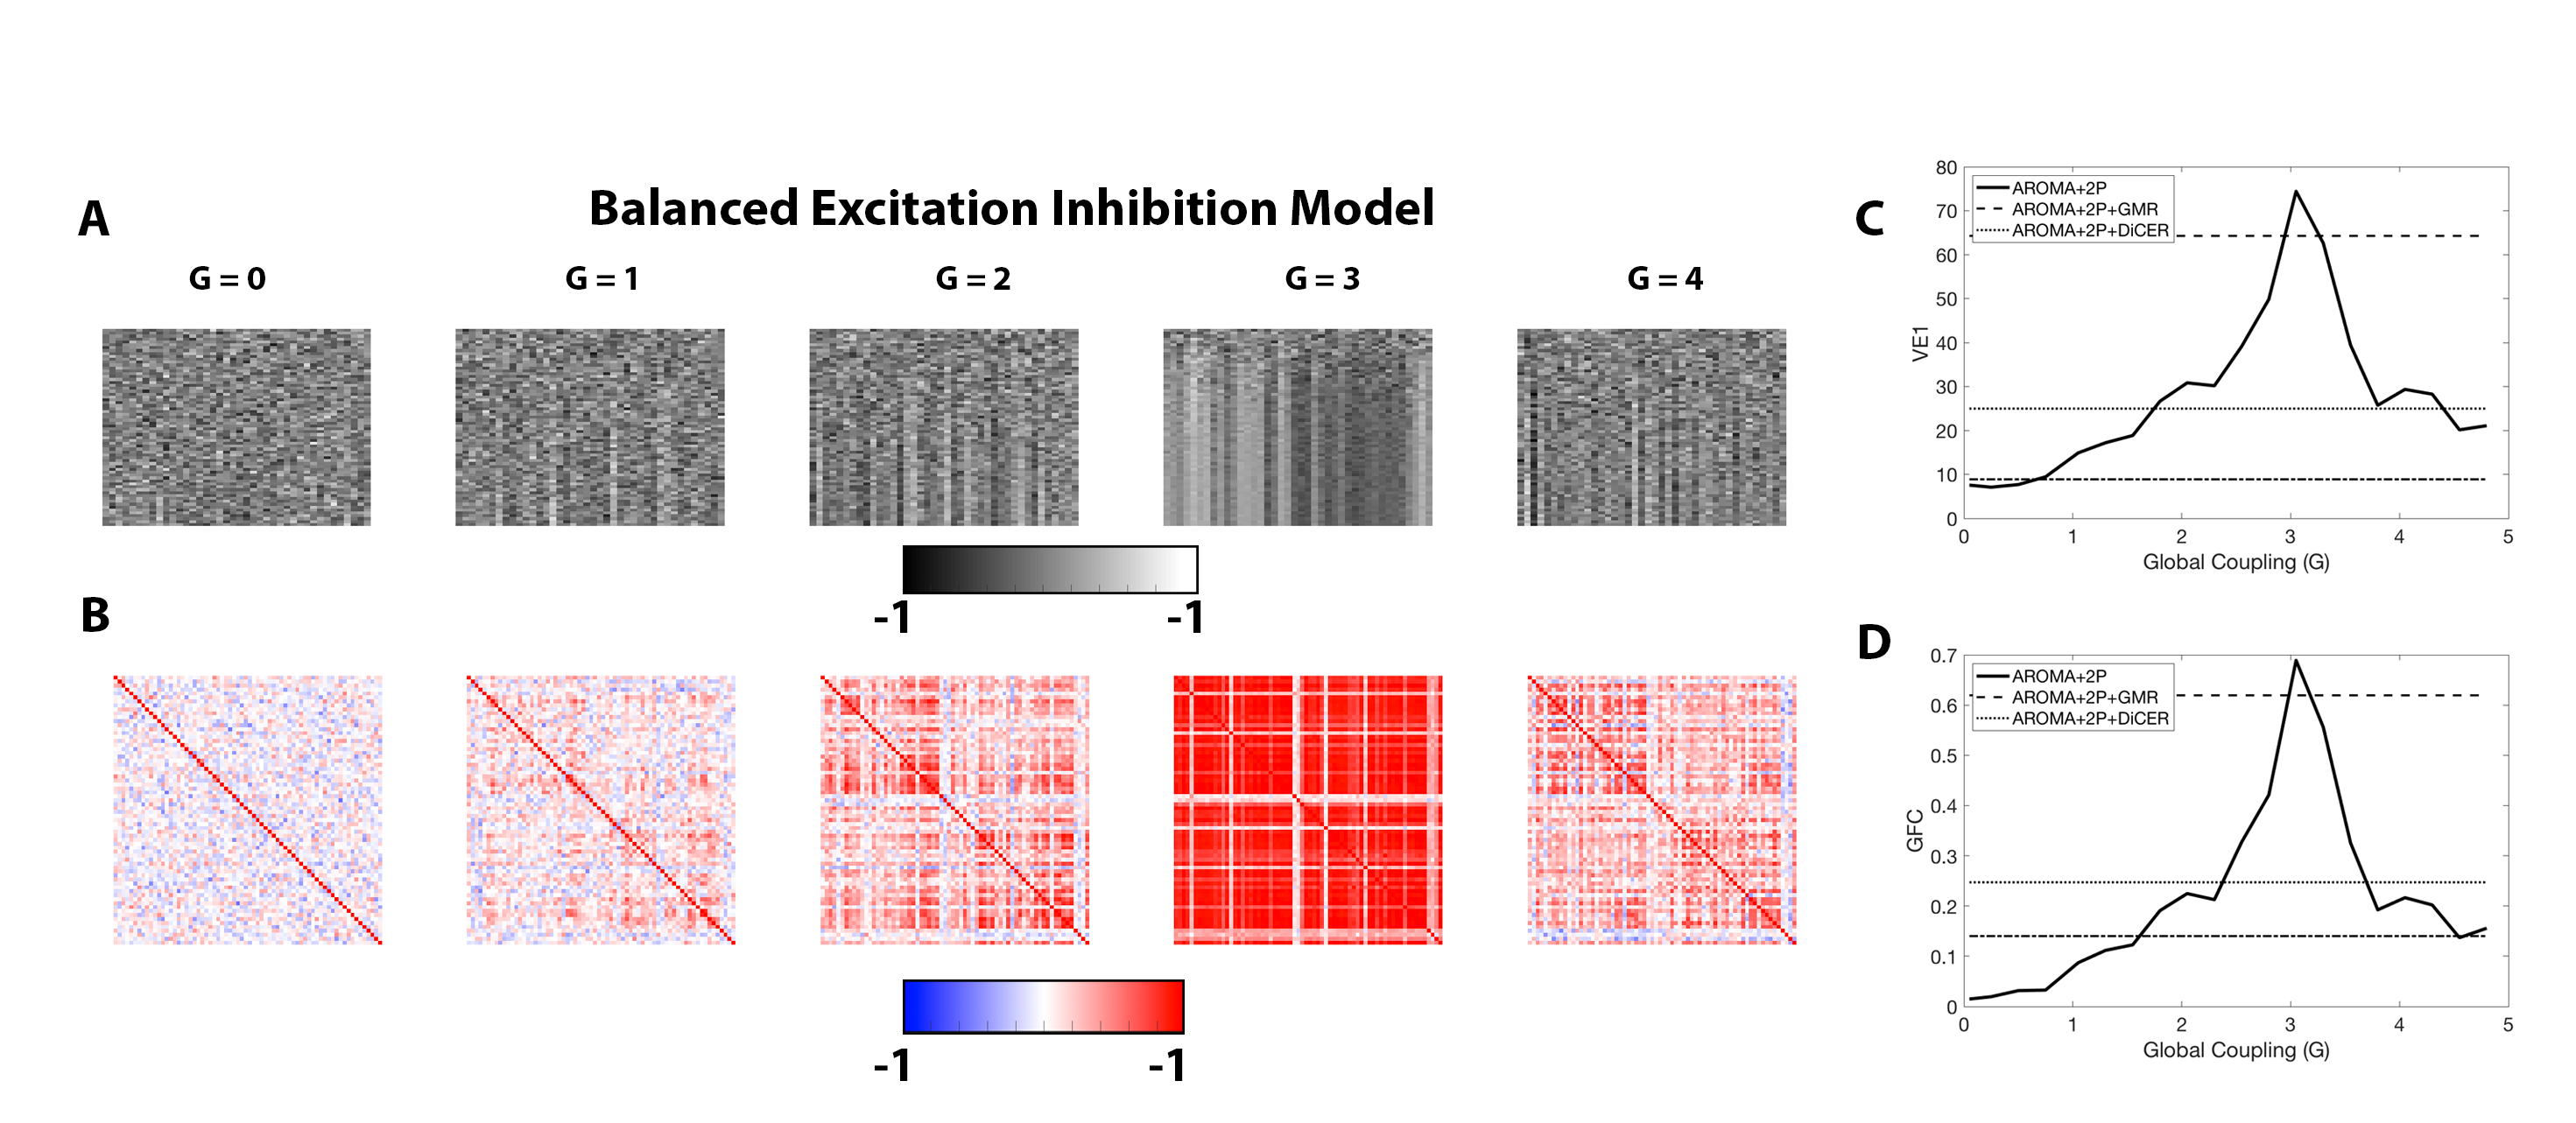
\includegraphics[width=1\textwidth]{figs/BEModel.png}
\caption{Wide spread deflections in the Balanced Excitation-inhibiton model. A B C D}\label{fig:BalancedEI_G}
\end{figure*}

\begin{figure*}[ht!]
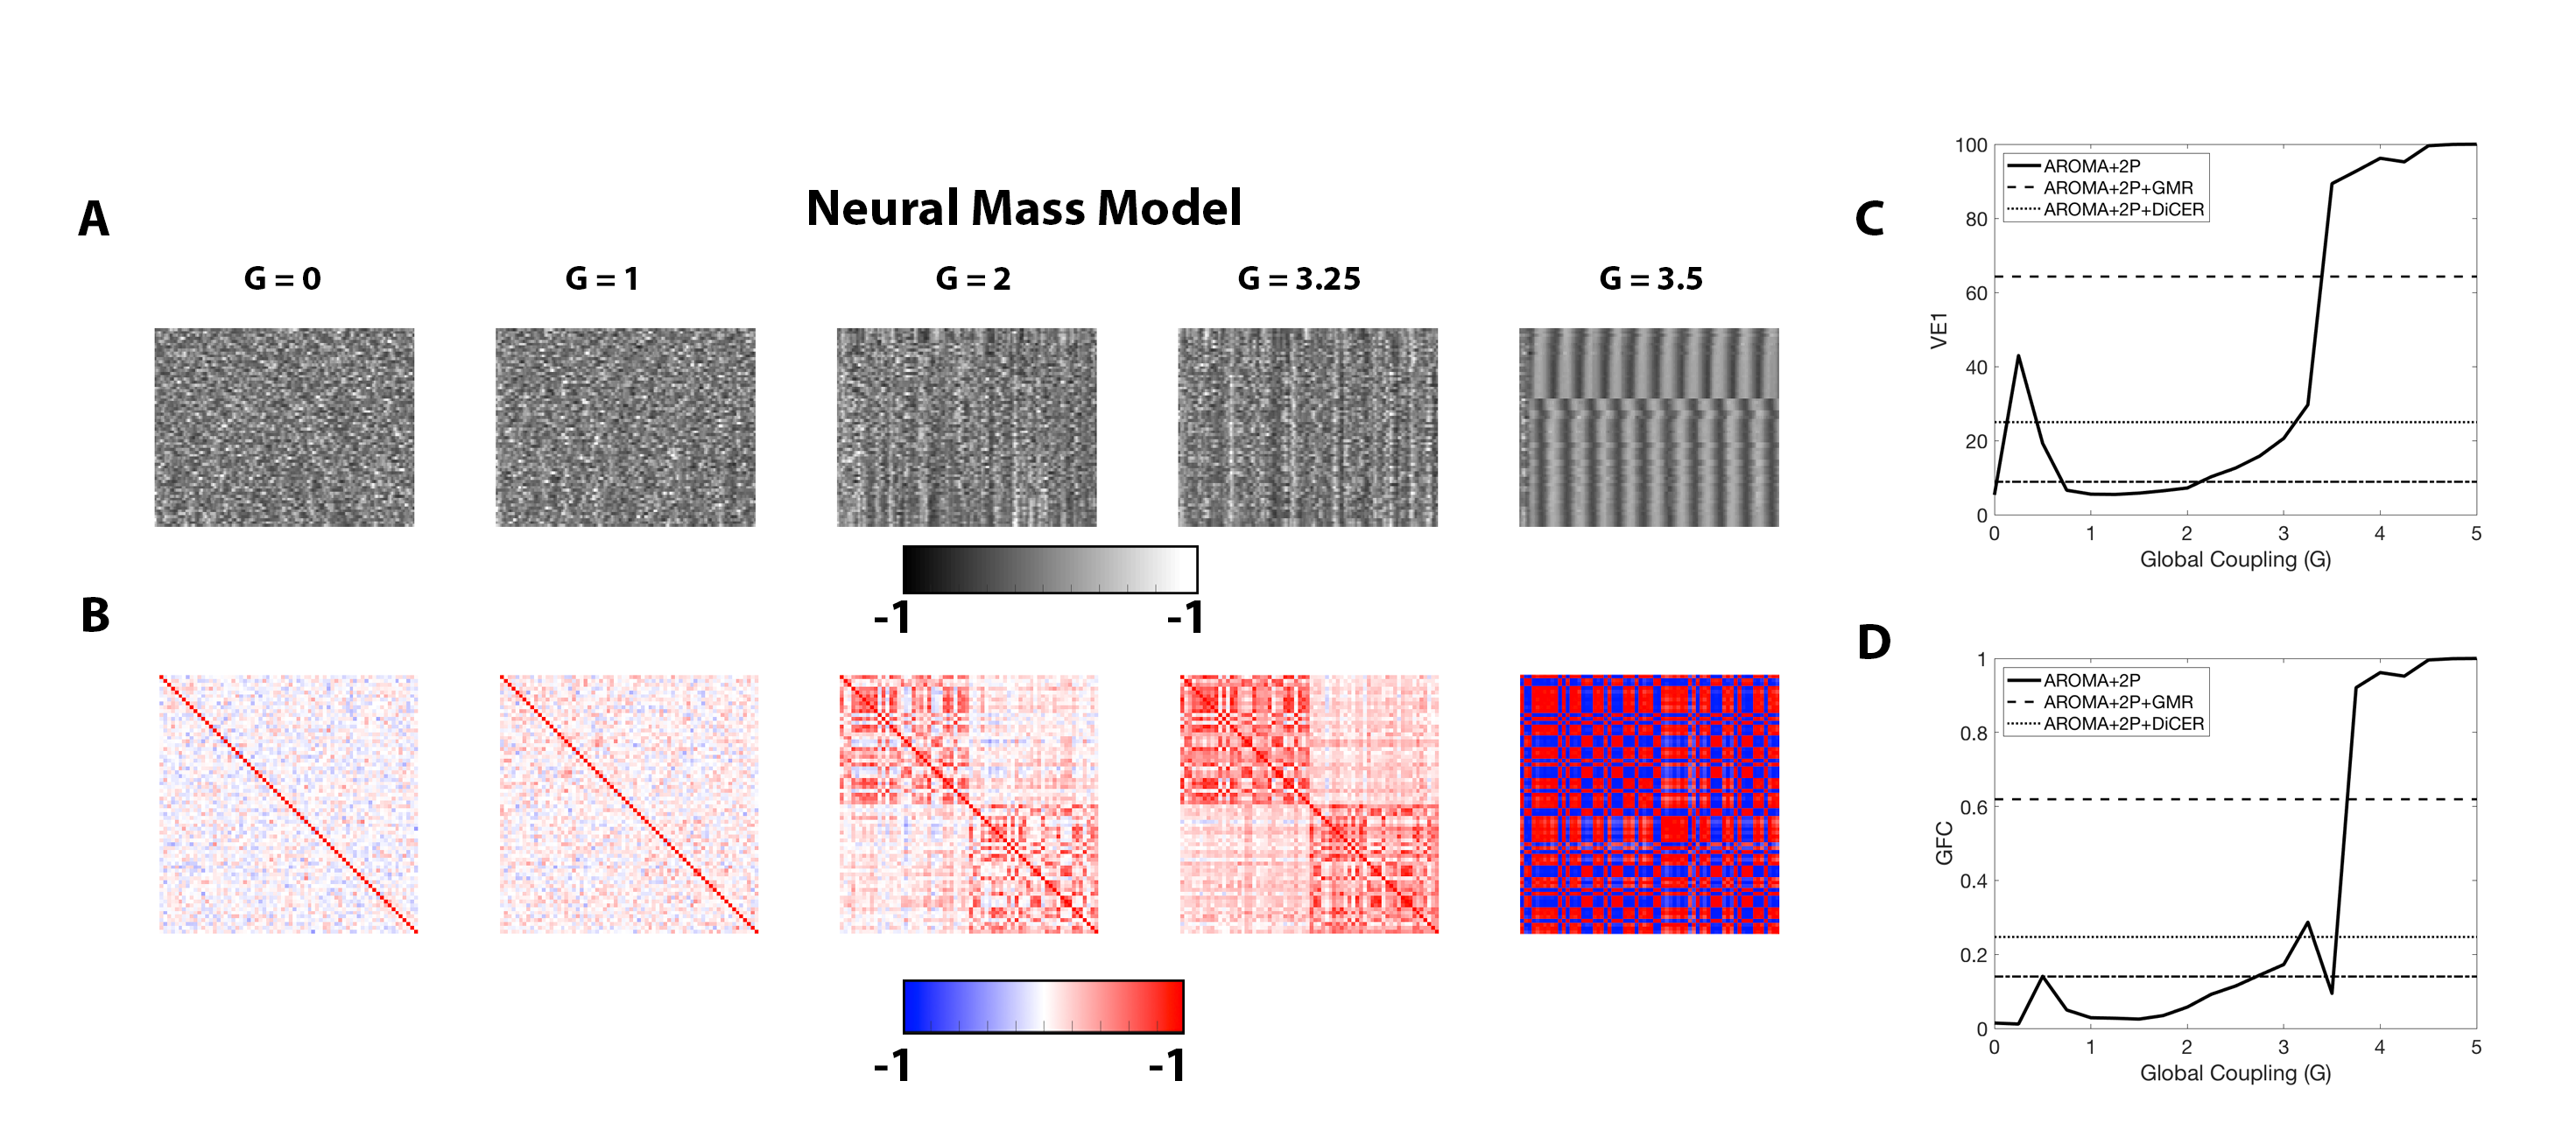
\includegraphics[width=1\textwidth]{figs/BTFImage.png}
\caption{Wide spread deflections in the neural mass model. A B C D}\label{fig:NM_G}
\end{figure*}

\begin{figure*}[ht!]
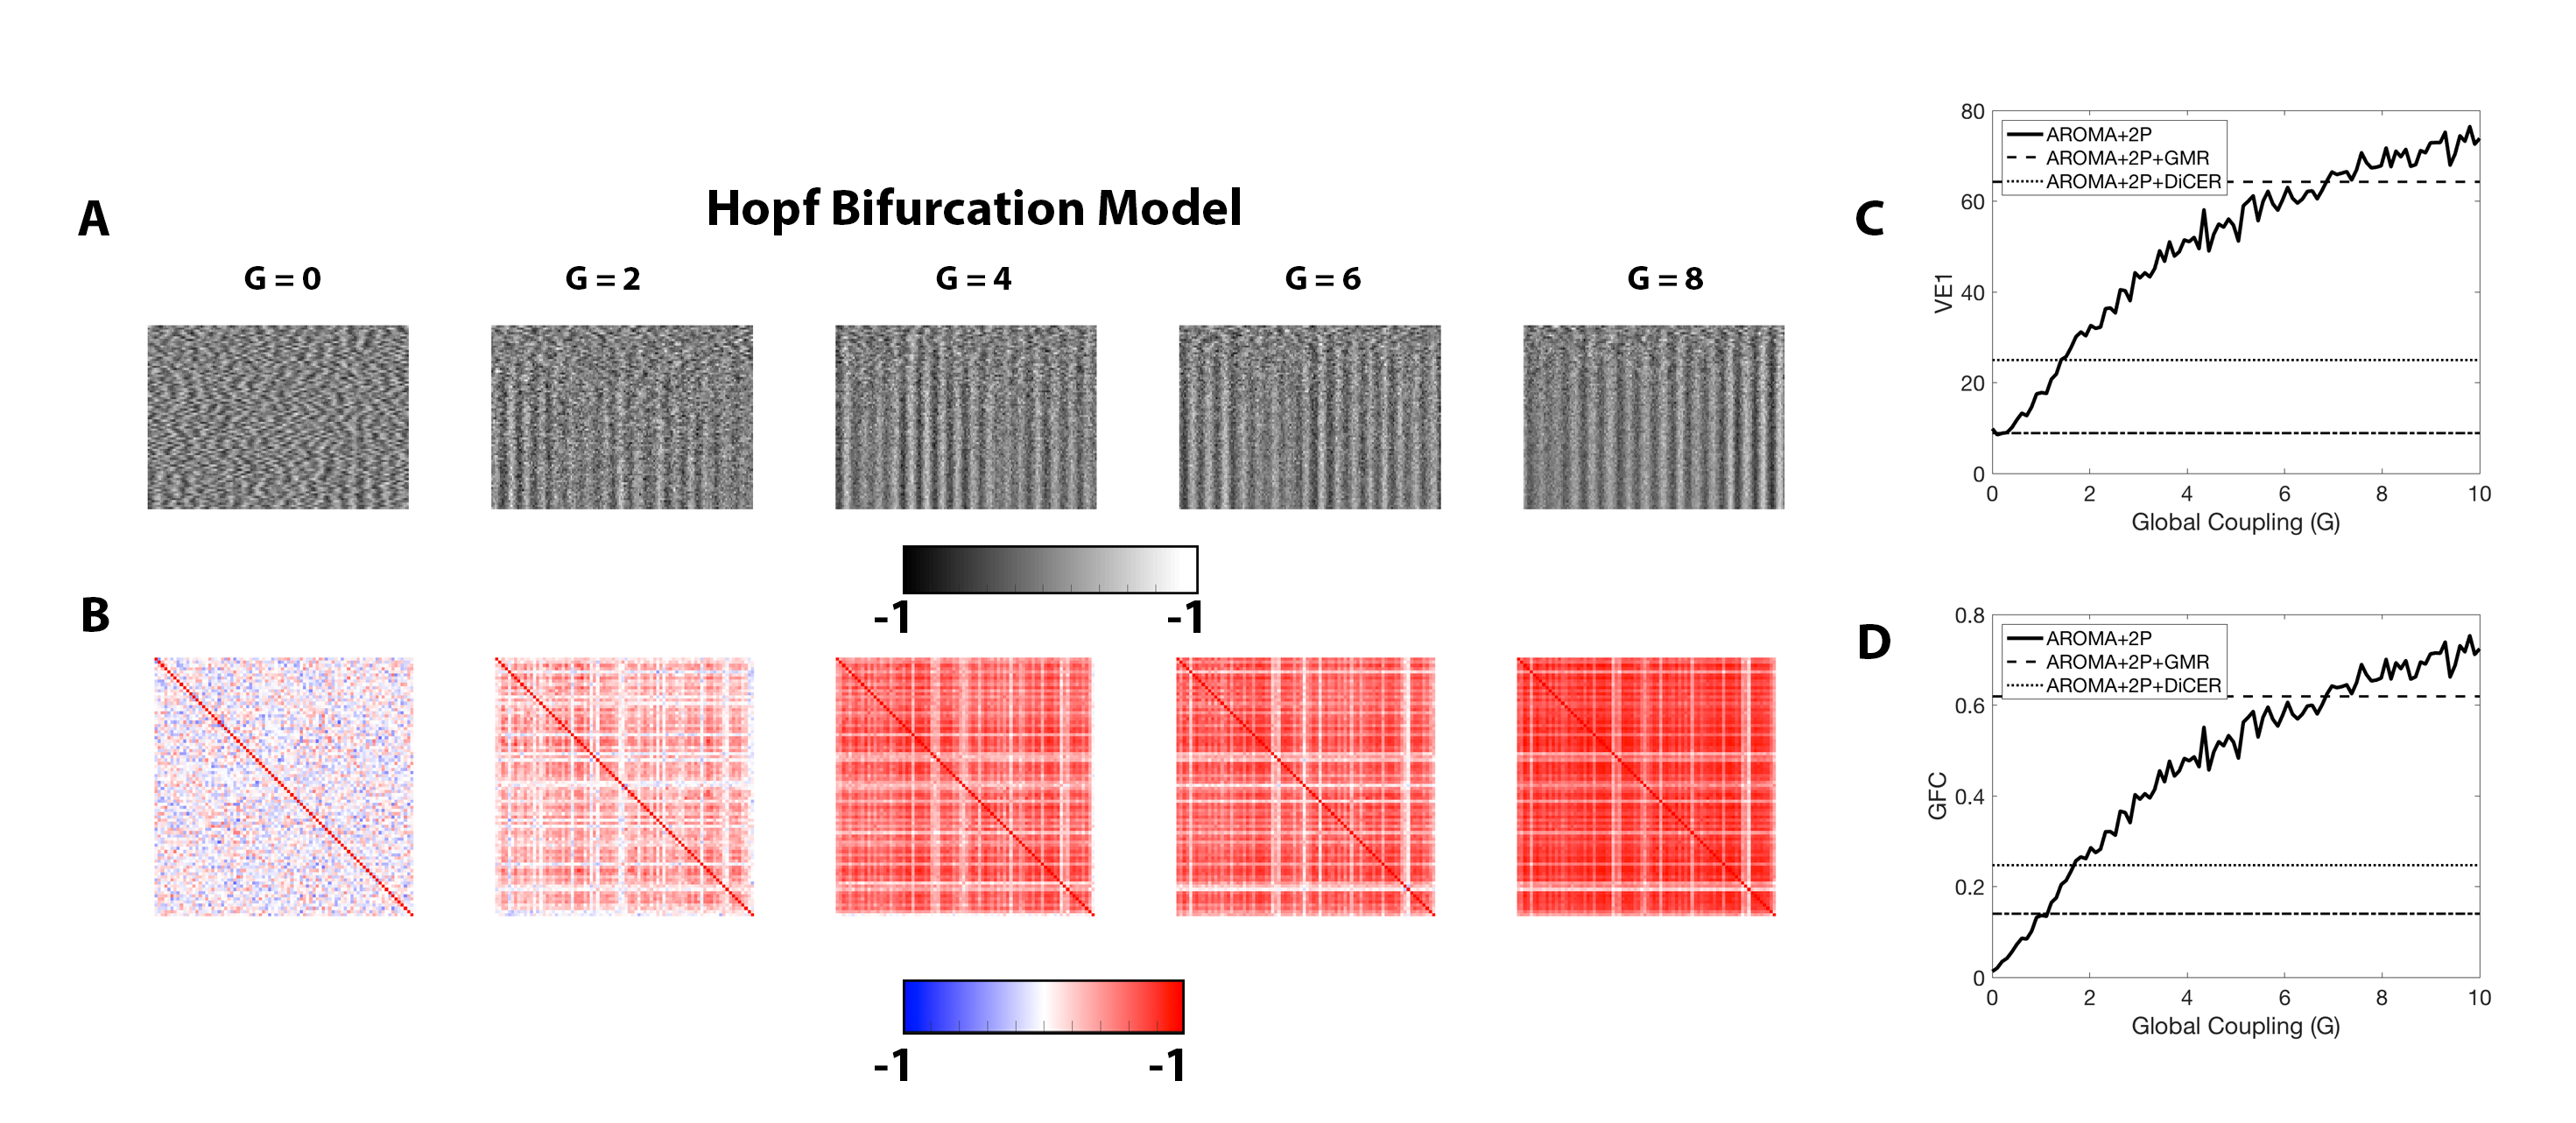
\includegraphics[width=1\textwidth]{figs/HopfImage.png}
\caption{Wide spread deflections in the Hopf Bifurcation model. A B C D}\label{fig:Hopf_G}
\end{figure*}


The above results indciate that data with WSDs requires models to be biased toward the synchronized regime, whereas data with reduced WSDs push data to the unsynchronized regime (i.e. lower $G$). We can explore this issue further in the highly synchronized regime, and the weakly synchronized regime. Firstly, models within the synchronized regime appear to have a globaly coherent signal is present in the spatiotemporal carpet plots as visually expressed by the large vertical stripes in Figs~\ref{fig:BalancedEI_G}~A,\ref{fig:NM_G}~A,\ref{fig:Hopf_G}A with $G=3,3.25,2--8$ respecively. If we were to model this behaviour explicitly, we first note that in all three models the local dynamics at node $i$ are modulated by the influences owing to the sum (or mean) of the neighbouring nodes weighted by $C$ i.e. by a general factor
\begin{equation}
G\sum_jC_{ij}f_{j}(t),
\end{equation}
where $f_{j}(t)$ is a general term that describes some output node $j$ expressed to node $i$ which in most models is the dynamics of excitatory population at node $j$. Thus, if all nodes shared a common signal $\sigma(t)$ the dynamics at node $i$ will be modulated by this common factor and a local Gaussian noise term $N(0,1)$ (owing to noisy inputs in all the three models) expressed as:
\begin{eqnarray}
B_i(t) &=& \alpha N(0,1) + G\sum_jC_{ij}\sigma(t),\\
	   &=& \alpha N(0,1) + GD_{i}\sigma(t),
\end{eqnarray}
where $D_i$ is the node degree, and $\alpha$ determines the strength of the noise term which we set at $\alpha=1/2$. When we use the common signal as the mean signal of sub-10274, this noisy degree model in Fig~\ref{fig:NDM_G} can reproduce carpet plots and FC matrices similar to the preprocessing pipeline ICA-AROMA+2P with $G=4$. Therefore, we note that a model of the global signal modulated by node degree is roughly equivalent to highly synchronized models of rsfMRI, and is well correlated  to the balanced to the Balanced Excitation Inibition model ($r=0.99$). (think about how this fits in..)

\begin{figure*}[ht!]
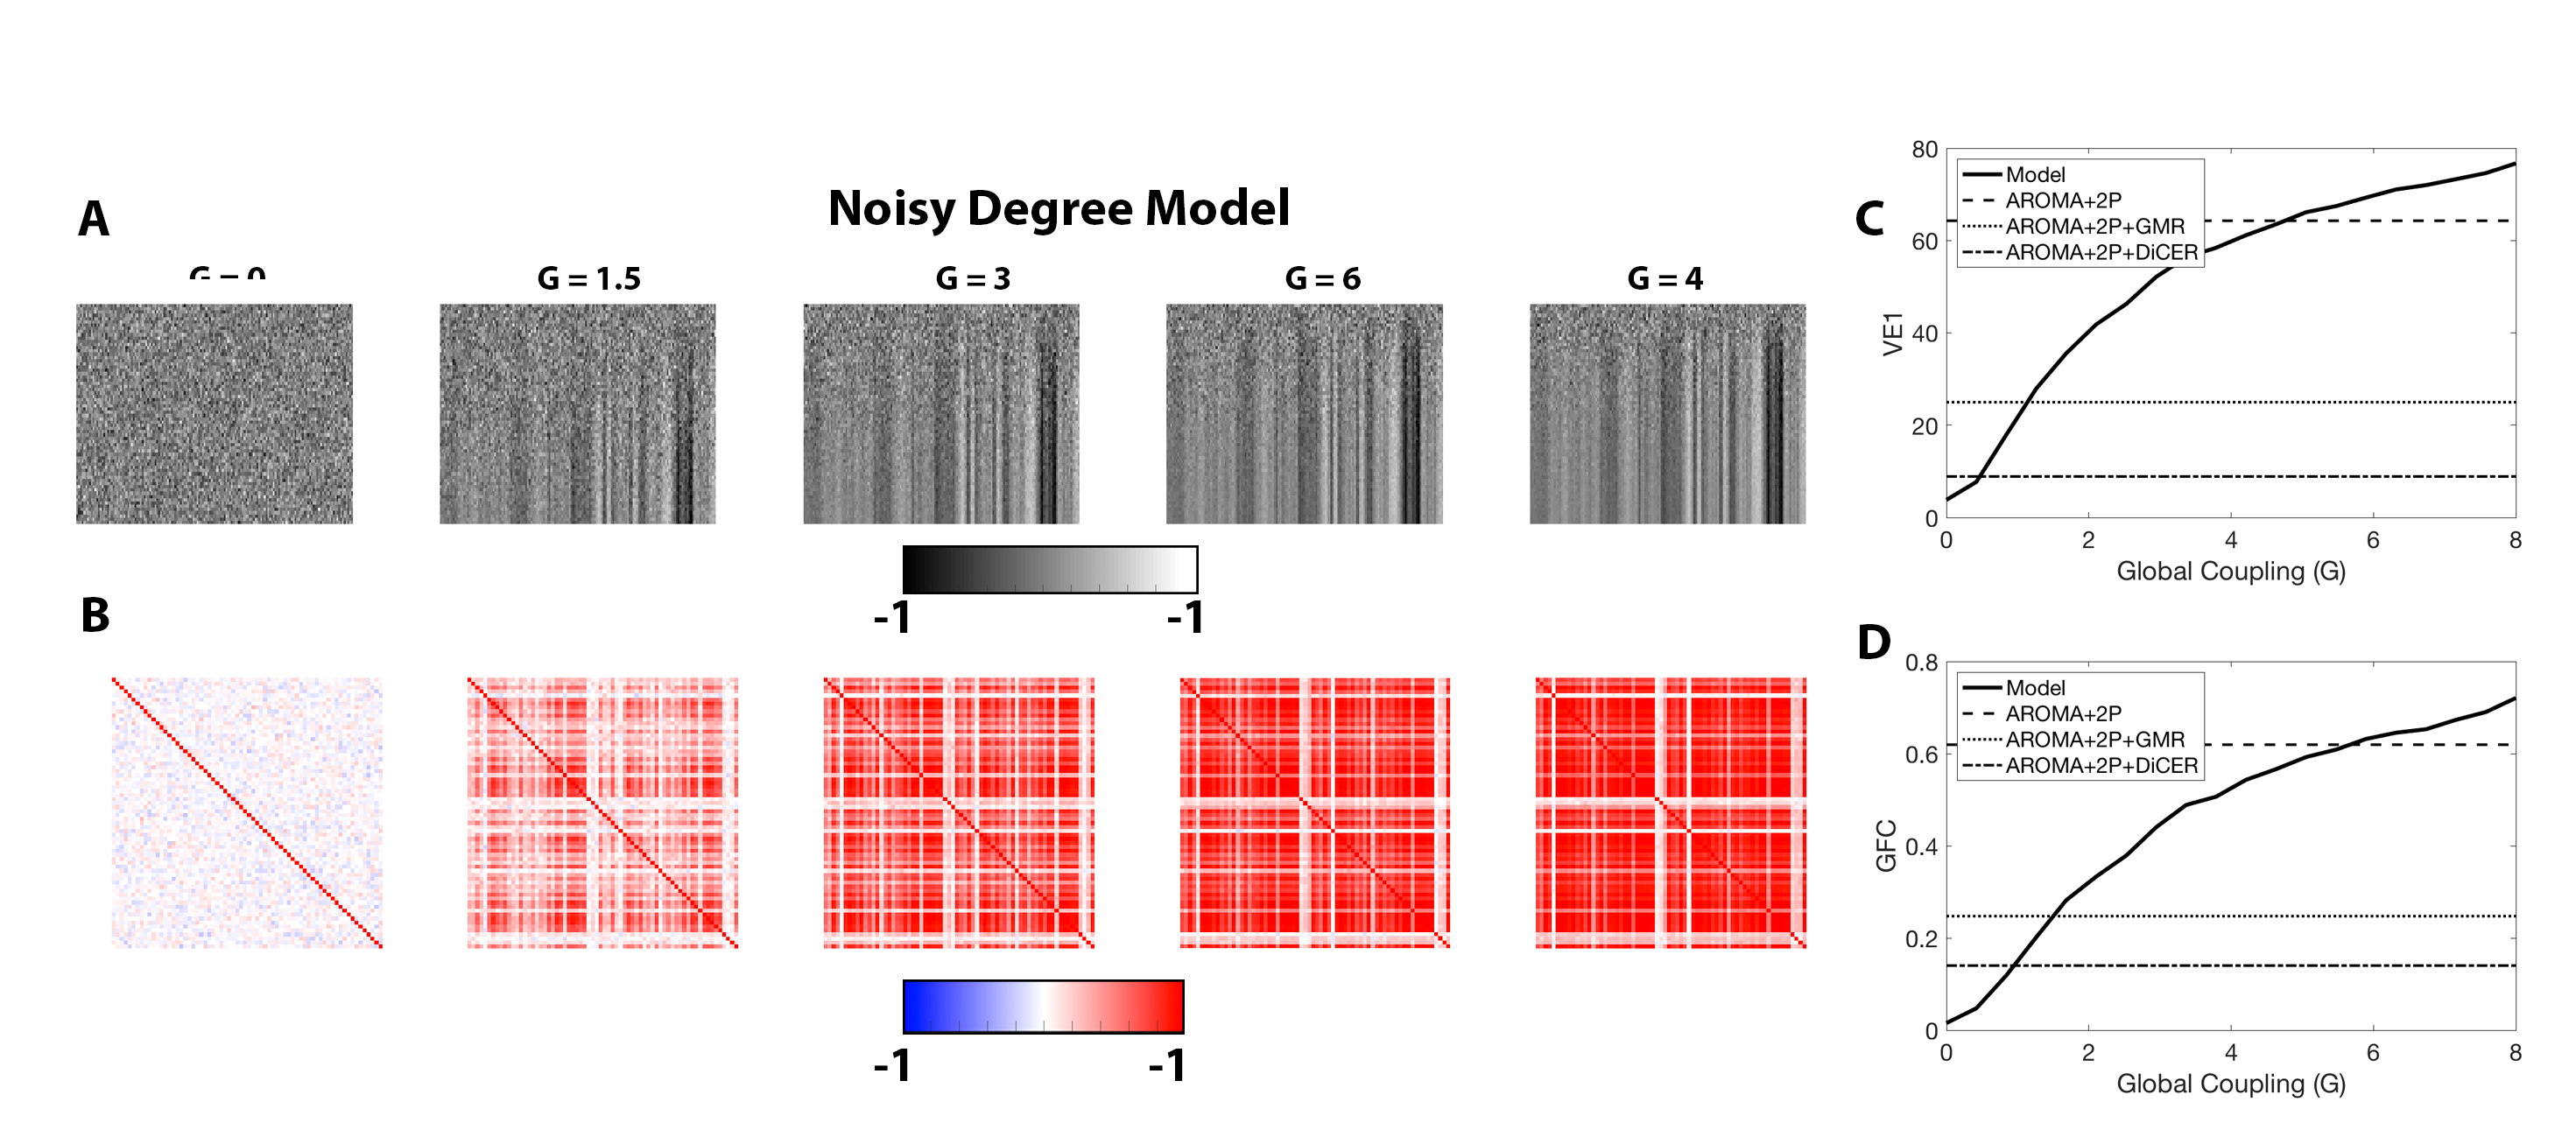
\includegraphics[width=1\textwidth]{figs/NDMModel.png}
\caption{Wide spread deflections in the Noisy degree model. A B C D}\label{fig:NDM_G}
\end{figure*}

Secondly, in the weakly synchronized regime, there are fewer WSDs and there is closer match with that undergoing GSR or DiCER. However, within the experimental fMRI literature, a key argument against the use of GMR is that it may remove neurally related WSDs. Here, the presented models simulate globally coherent neuronal fluctuations, thus a key question is what remains post GSR. Following GMR, we see three types of artefactual effects in the three presented models in Fig.~\ref{fig:GMRModels}. For low $G$, WSDs are removed lowering VE1 and GFC (we exclude the noisy degree model as by construction, most of the signal is removed post GMR). This effect is present however, for all $G$ for the Hopf bifurcation model. Secondly, When there is a globally coherent signal that is delayed between nodes - such as those imposed by a travelling wave (Roberts et al.) - the mean signal can does not capture the WSD such as in the neural mass model for $G=3.5$ as in Fig.\ref{fig:NM_G}~A thus leaving WSDs post GMR in Figure.~\ref{fig:GMRModels}~E,F. And finally, a residual artefactual signal can be left behind following GMR for the balanced EI models for $G=3$. In all models and global parameter variations, only the neural mass model for $G=2-3$ and the balaneced EI model for $G=2,4$ leaves residual structure in the FC matrix, indicating residual modulations above globally coherent ones. These are visual comparisons provide indications of the artefacts and FC matrix structure, quantiative comparisons with rsfMRI are described in the next section. 


\begin{figure*}[ht!]
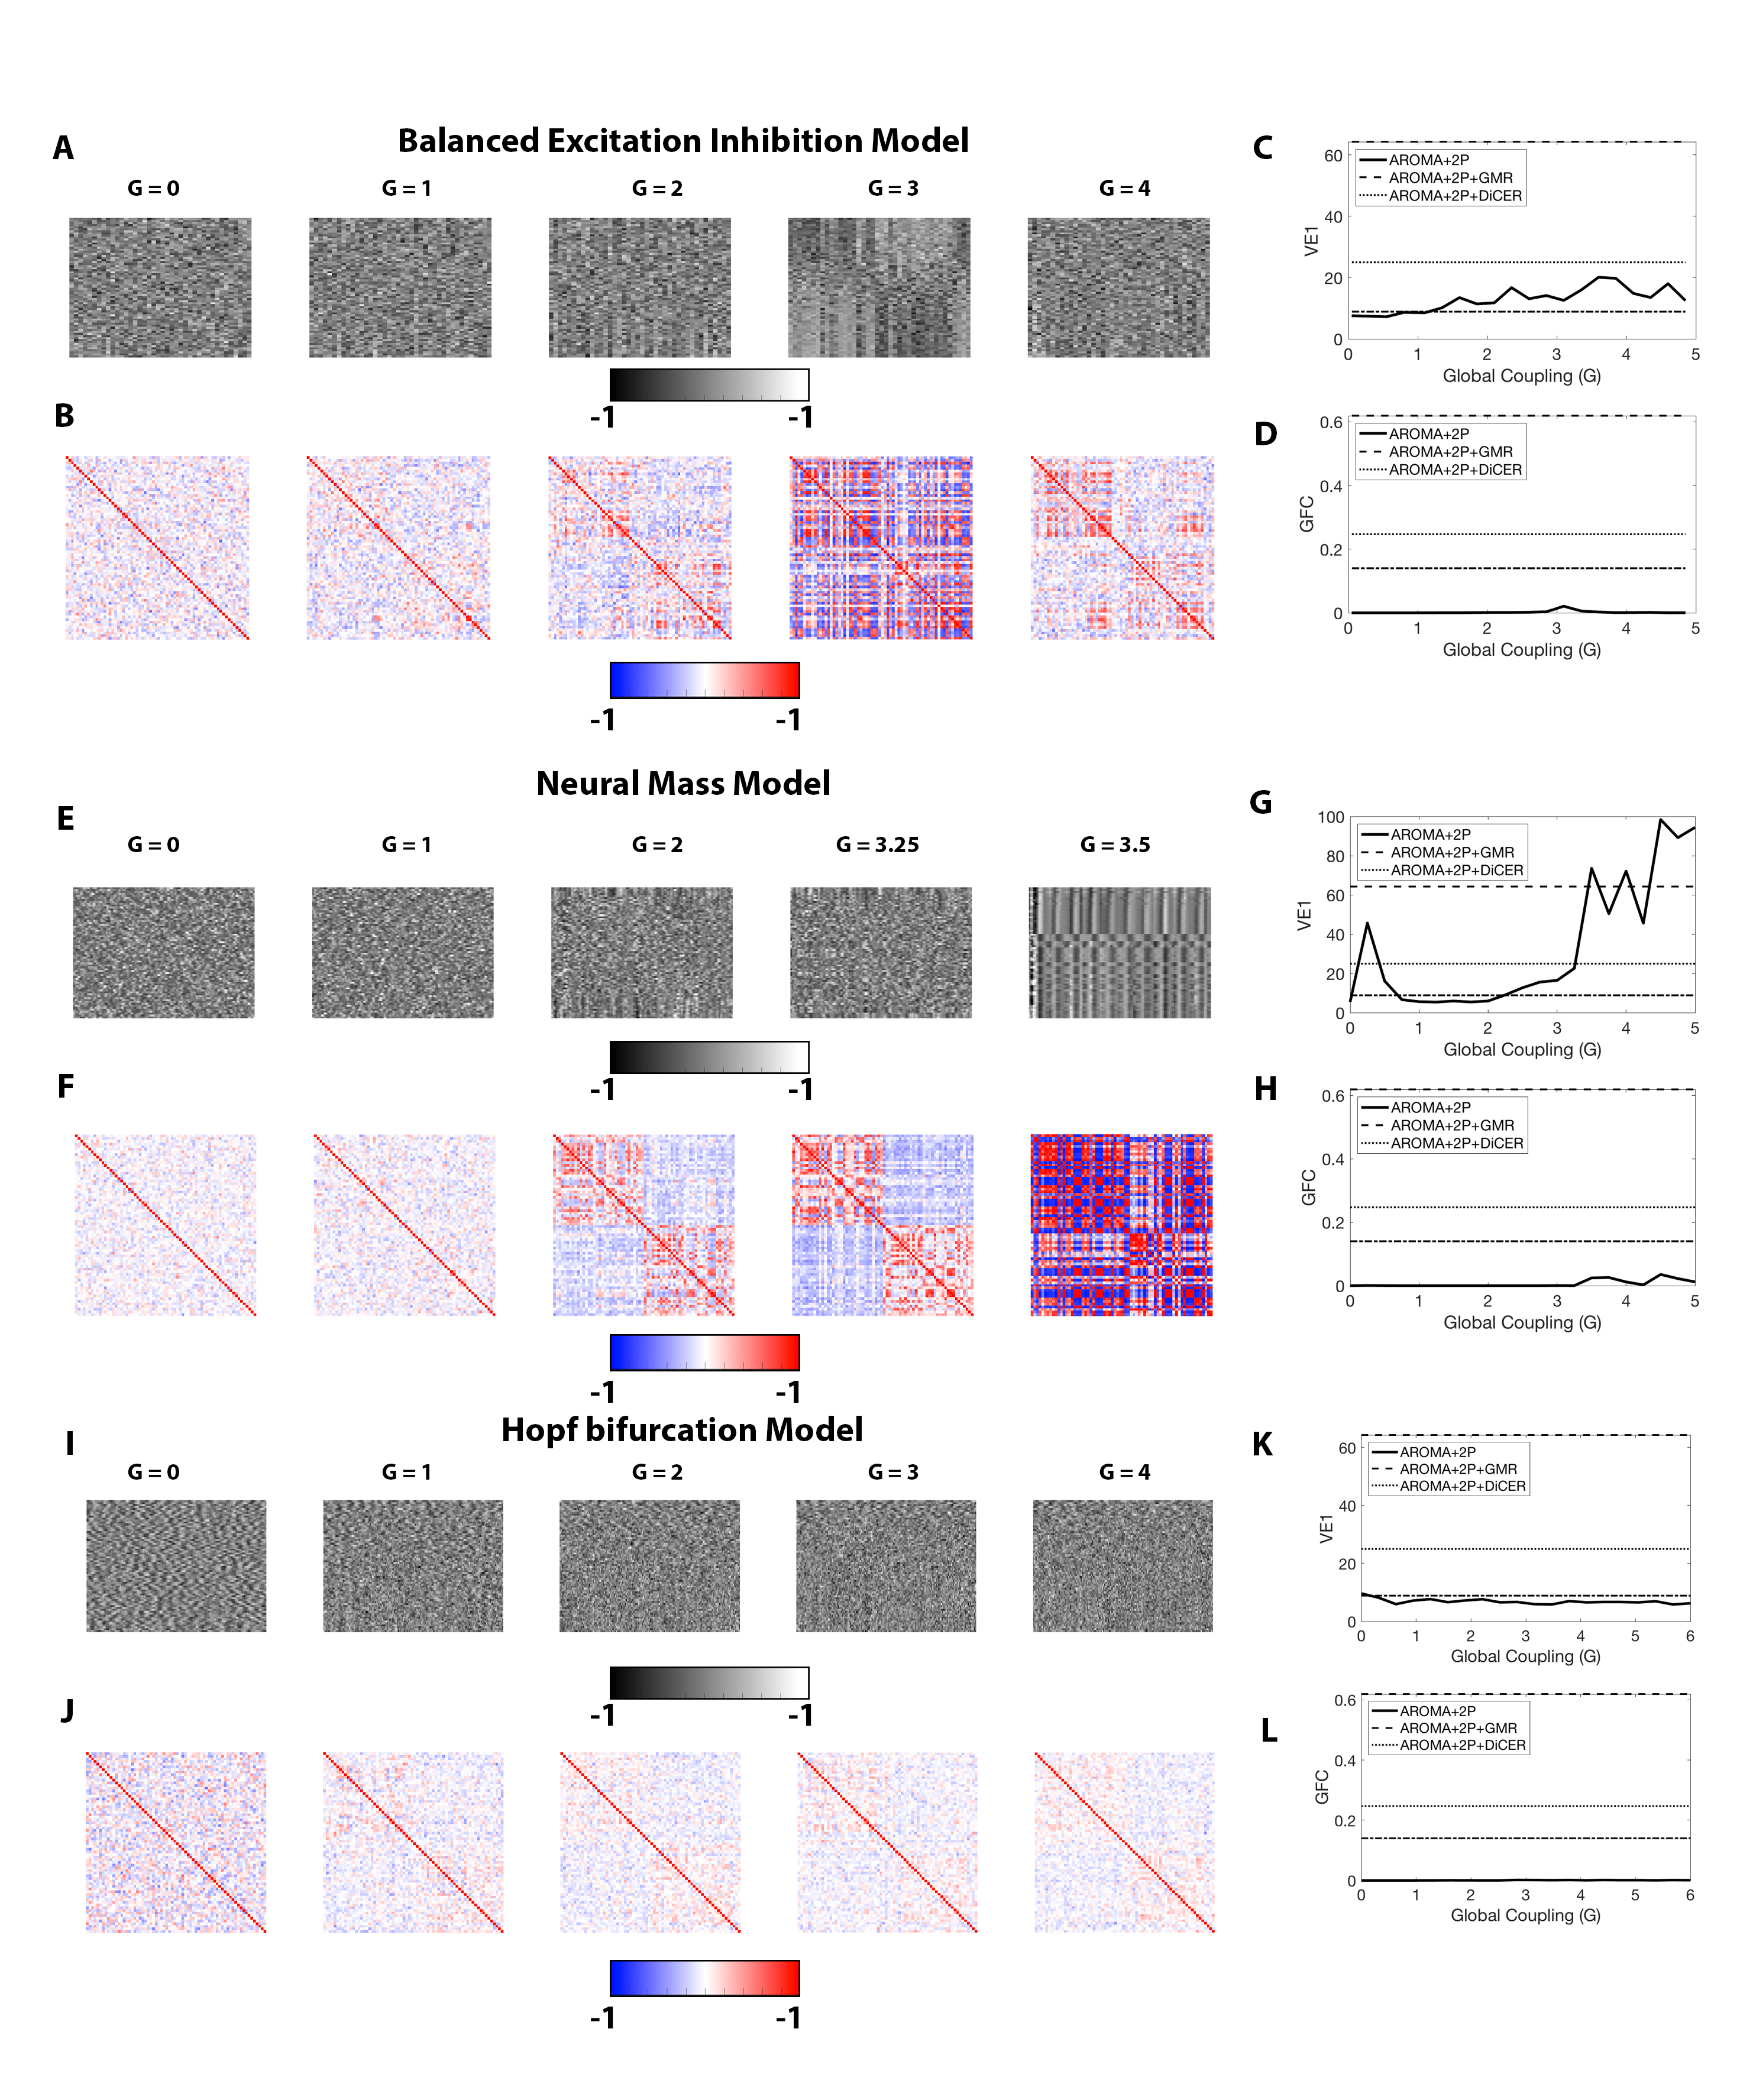
\includegraphics[width=1\textwidth]{figs/GMRModels.png}
\caption{GMR models}\label{fig:GMRModels}
\end{figure*}

The above results relate to the appearance WSDs visually in the spatiotemporal characteristics and on FC matrcies, improvements in rsfMRI mdoelling is the focus on dynamic measures of functional connections. Here, we examine dynamic functional connectivity in a similar fashion to above.

We calculate the DFC and find that
% We find that X and Y. 

% The two above metrics can then be used to analyze the models themselves. 


% The above results relate to static measures of dynamic activity, of course an additional measure is to use a dynamic measure - dynamic functional connectivity. 

% + Then talk about FCDs and match to data. 


\subsection*{WSDs affect model fits}

With a characterization of the wide spread deflections in rsfMRI data and modelling, we can now explore how well these features correspond to quantitative model fits.



Also have to fix for BTF (need to run many simulations)

Show Fit values, FCD values and DMN type of figures for all of them

Then talk about this.

Then talk about improving the models with heterongeous parameters on A -- doesn't work.

Then talk about imrpovements with ANEC, it does work but at WHAT COST??!?!?

Thats it. 



3. How this effects both FCs and FCD show this for the optimal settings.

Need to talk about the differences in the fittings on both FCD and FC, say that we previously showed how different coupling changes WSDs and then results change too.


3++ Influence on heterogenous parameters. - talk about ways to combat this. 

Three datasets show this - distribution of the G optimal values
4. Derivation of the Noisy-degree model, show on the B-EI model relative to GSR (in a figure with plots and things)

we can derive this model - interesting relationship need to understand it - is it also related to ROI size? not sure.

5. Then talk about improvements -- ANEC can do so. 


+First show some carpet plots, talk about how these carpet plots show the level of coherent data, talk about how they represnet differenet levels of coherence and how they effect FC, dynamic FC.


The problem with WSDs in data (and we dont correct for them) is that we then build and focus on models that also have large WSDs. 

Maybe then here we could show something with that on purpose.......

We have simple measures there. 


We first have a summary of all the data, and how to interpret these (important points to highlight).

Before modelling - we urge modellers to understand these effects. 

Show the results + show carpet plots and stuff

Say that WSDs influence all of it


+++ Heterogeneity, things that can be done.

+++ ANEC 



\section*{Discussion}
Global signal - noise or what? the problems within models. 

\subsection*{Evidence against using data without some denoising} 
Need to discuss that a common reason not to use GMR (or even other WSD reducing types of analysis) is that it will impact neuronally driven WSDs - a feature in many models (as seen above). However models may just be fitting this and nothing else if theya re not careful. 

\subsection*{The Balloon model} 

A common forward model in the literature is to use the Balloon-windkessl model to simulate forward model dynamics. Although its use is common, a number of studies has invalidated the use of the Balloon model - namely the non-existence of the venous balloon. Although, the Balloon model may capture non-linear properites of the BOLD response in resting state it is likely that this is not achieved. Therefore we advise against the use of this model. 

\section*{Notes}
+ Parcellation discussion increase

\section*{Acknowledgements}


\begin{acknowledgements}
AF was supported by the Australian Research Council (ID: FT130100589), National Health and Medical Research Council (NHMRC; ID: 1104580), and the Sylvia and Charles Viertel Charitable Foundation. The authors thank Stuart Heitmann for support of the Brain connectivity toolbox, and Christopher honey and Olaf sporns for sharing code. 
\end{acknowledgements}

\section*{Bibliography}
\bibliographystyle{benbibstyle}
\interlinepenalty=10000
\bibliography{GSR_references}

%% You can use these special %TC: tags to ignore certain parts of the text.
%TC:ignore
%the command above ignores this section for word count
\onecolumn
\newpage


%  this study is going to bridge that gap by using biophyiscal models of the certain kind. Will show the effects that WSDs provide, showing how WSDs can influence findings and corrupt the work. Here, we bring into question the role and urge QC-FC type of measures as well as carpet plots. We end with a note on how things can be improved with heteroengous models but at the cost of model complexity. 


% What i think is instead cool is to have two different sections, 

% firstly show the effects that different preprocessing has and relationships to data. 
% We find a very important influence of global fluctuations and state that without careful consideration we are only really fitting this large oscillations. We can just use the ND model instead.

% Then say from a modelling point of view this is very attractive as if there is a complex network resting state fMRI can be seen as small pertubations, and from a dynamic perspective this allows a large amount of dynamics that are applicable from other sources.



% Things to talk about in the introduction:
% + General large-scale network modelling
% + What is being fitted (rsfMRI correlations)
% + Problems in the field regarding Large-coherent structures
% + Largely ignore by the modelling community (no real discussion of this)
% 	-- Discussion more on GSR vs noGSR (Hannes paper, Messe et al as well)
% + If we treat model simulations as numerical experiments we can then understand the simulated data in the same light
% + Summary of the rest of the paper - starting with a special case of the balanced EI model, using the tools and the models under different preprocessing lights. Introduce the noisy-degree model (could be something that is really interesting on its own, but it does not need anything else.)


% Over the last two decades, functional magnetic resonance imaging (fMRI) has heavily focused on understanding the brain "at rest". 
% Imaging the brain at ``rest'' ,or more accurately task-free,   is thought to accentuate the brain's complex functional networks (REFS) under the premise that key networks of brain function have a correlated structure (REFS). 
% This paradigm has lead to the discovery of robust resting networks that are altered once the brain is engaged tasks, are altered in disease, and consistent across populations as well as species. 
% These discoveries have lead to various questions -- such as what is the role of these networks? what are the key elements are altered during disease, and importantly how stucture shapes cortical function.



% Talk about the tools to de-noise: popular methods are typically seen in the following light - take estimates 


% This crisis in the experimental and data analysis litertaure has largely been ignored in large scale biopyhysical modelling. In This crisis


% Hence, this has been a large focus of large scale brain dynamics. 

% Hence, there has been a large focus to understand the data acquired from this paradigm 

%  although easy to acquire, has presented a number of challenges there has been a paradigm shift to stray away from understanding task specific brain activity to 


% Functional magnetic resonance imaging (fMRI) of the brain at rest has brought upon a plehtora of studies to understand the correlational structure of cortex. A number of studies have used this resting paradigm 


% Need to mention that very bad prepro has been used. 

% \section*{Methods 1: Experimental data}

% \section*{Methods 2: Brain network modelling}
% generic theory:
% \begin{equation}
% 	\frac{d}{dt}z_{i}(t) = f(A,{\bf z}) + I.
% \end{equation}
% where $A$ is the structural connectivity matix 

% \section*{The premise: Resting state functional networks}

% Here talk about the results and what is extracted. Then talk about the modelling from structure to function, essentially what people have been doing. State that there has been success. 

% Then state the problems, and they have unfortunately been treated seemingly independently.

% Independent problems:
% From the modeling side: Homogenous vs heterogenous. Types of different dynamical mechanisms. Types of oscillatory models.
% From the data side: preprocessing, global signal regression? inter subject registration

% Fusion problems:
% Where worlds meet:
% Fitting models to data
% - Find fitting statistics FCD, FC, Correlations
% - Making inferences from data
% - GSR the assumption that it is the panacea. From a modeling perspective we are removing the global neural mode however this is NOT equivalent to what is happening, the reason is different. 

% Assumptions, that all problems listed above have been handled/sorted/agreed upon in the field. The question is how much does it matter? Here we will strive to show the problems associated with it -- FC and FCD are not enough as many models can fit the data. Show in a case study in a very simplified model. We show how much Global signal changes the fitting -- GSR is not adequate however. 

% Show that we are not ready yet to make robust inferences, we need better models and cleaner data.

% \section*{Theory and results}

% Add in stuff to do with 

% The problems with FC and FCD

% Definitions of data \\
% Definitions of global signals \\
% Definitions of models (heterogenous vs homogenous models) \\
% Show different candidates of metrics: FC,FCD and correlations.
% Show the different types \\

% \section*{Theory and predictions}

% How many sample points are needed?
% Perhaps something we should also ask is how much of the time domain needed for the functional connectivity emerge as a robust measure -- timings etc. Which edges take the longest.

% Perhaps we need a certainty. 

% \section*{Results from modeling:}
% Need to have a table here

% \section*{ways to improve things}
% We take correlations blindly in functional networks on large scale connectivity. Perhaps however we need estimates of uncertainty on each node -- this way the model does not have to prove the existence of this connection. 

% How robust are connections to preprocessing methods and timing windows? Then fitting needs to work on this assumption.

% Heterogeneity is the answer. but preprocessing matters. 

% GSR is probably not the answer.

% ANEC

% \section*{Points that need to be discussed/mentioned here}

% There is a big divide between modeling and experimental expertise \\
% There is an assumption of quality on each side \\
% Preprocessing affects the model findings and interpretation \\
% Discussion of homogenous vs heterogenous models\\
% The balanced EI model shows although good fit without GSR, it unfortunately not so good. \\
% The interplay between theory and experiment. \\
% Does it matter? we have a test scenario SCZ vs CTL -- what are the differences? \\
% Models fit best with the worst kind of preprocessing.

% \section*{Discussion}

% What is actually being modelled? Is this brain function, or just a perturbation of a resting idled brain? This is not generalizable really. If one were to take a simple visual response what do we see? Should the models capture all this behaviour?

% We need better measures - FCD? not sure if this is enough, we need more stuff. Also need to have predictive validity. 


% also idea, shift the last few Gs stuff to negative see what GSR does to it.

\end{document}
